% !TEX root =  free234.tex
\chapter{Integrals} 
%
%\begin{center}
%  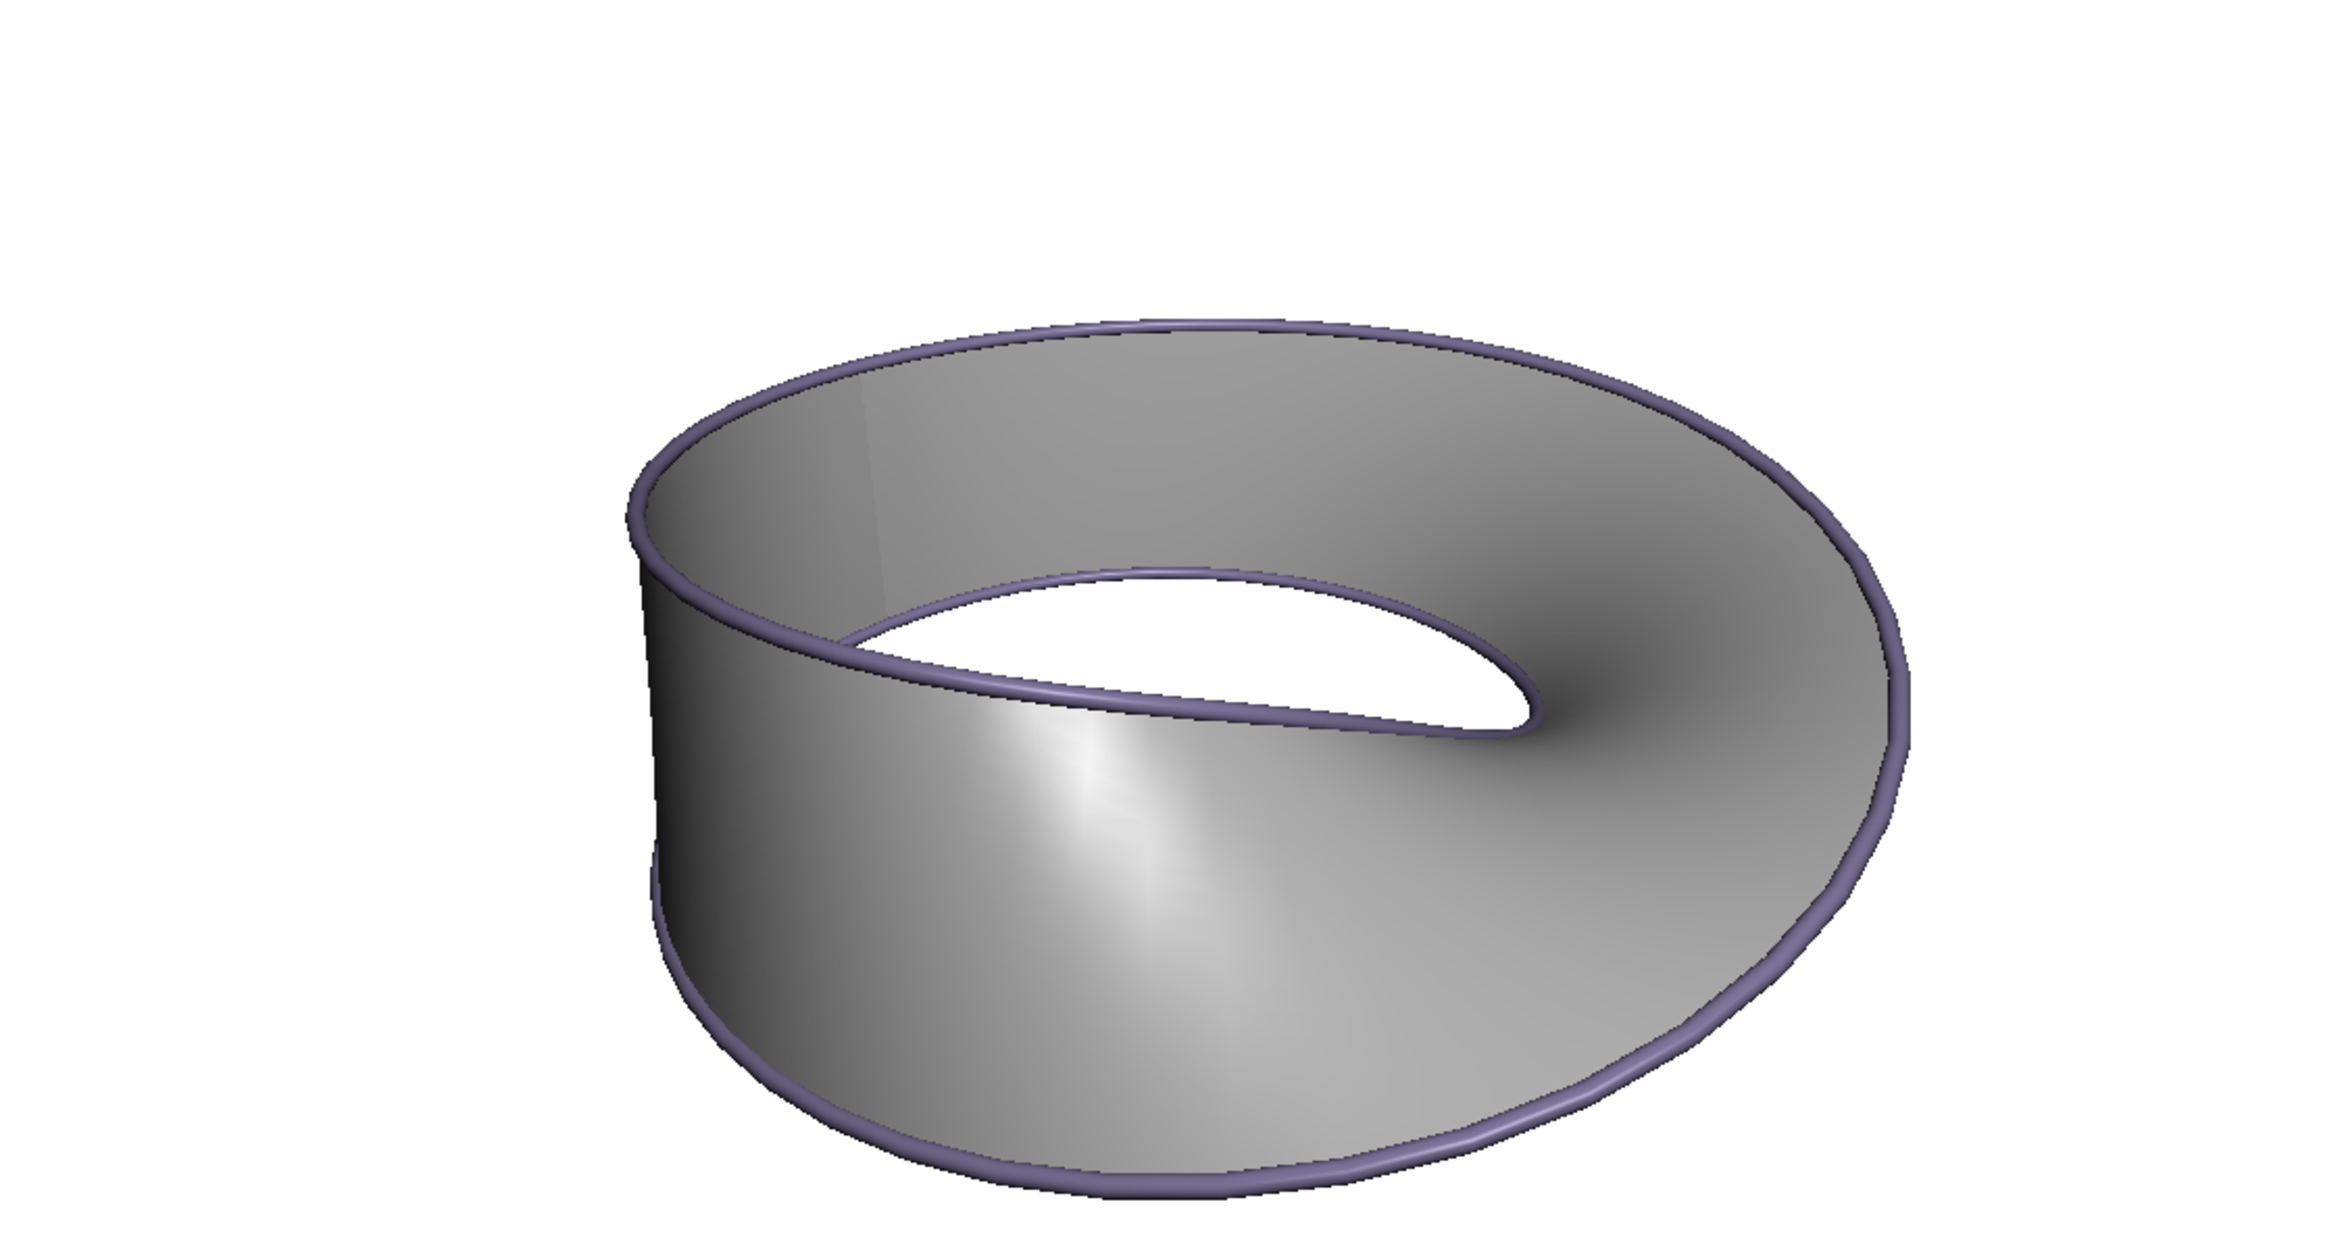
\includegraphics[width=3in]{Mobius_without_patches.pdf}\hfill
%  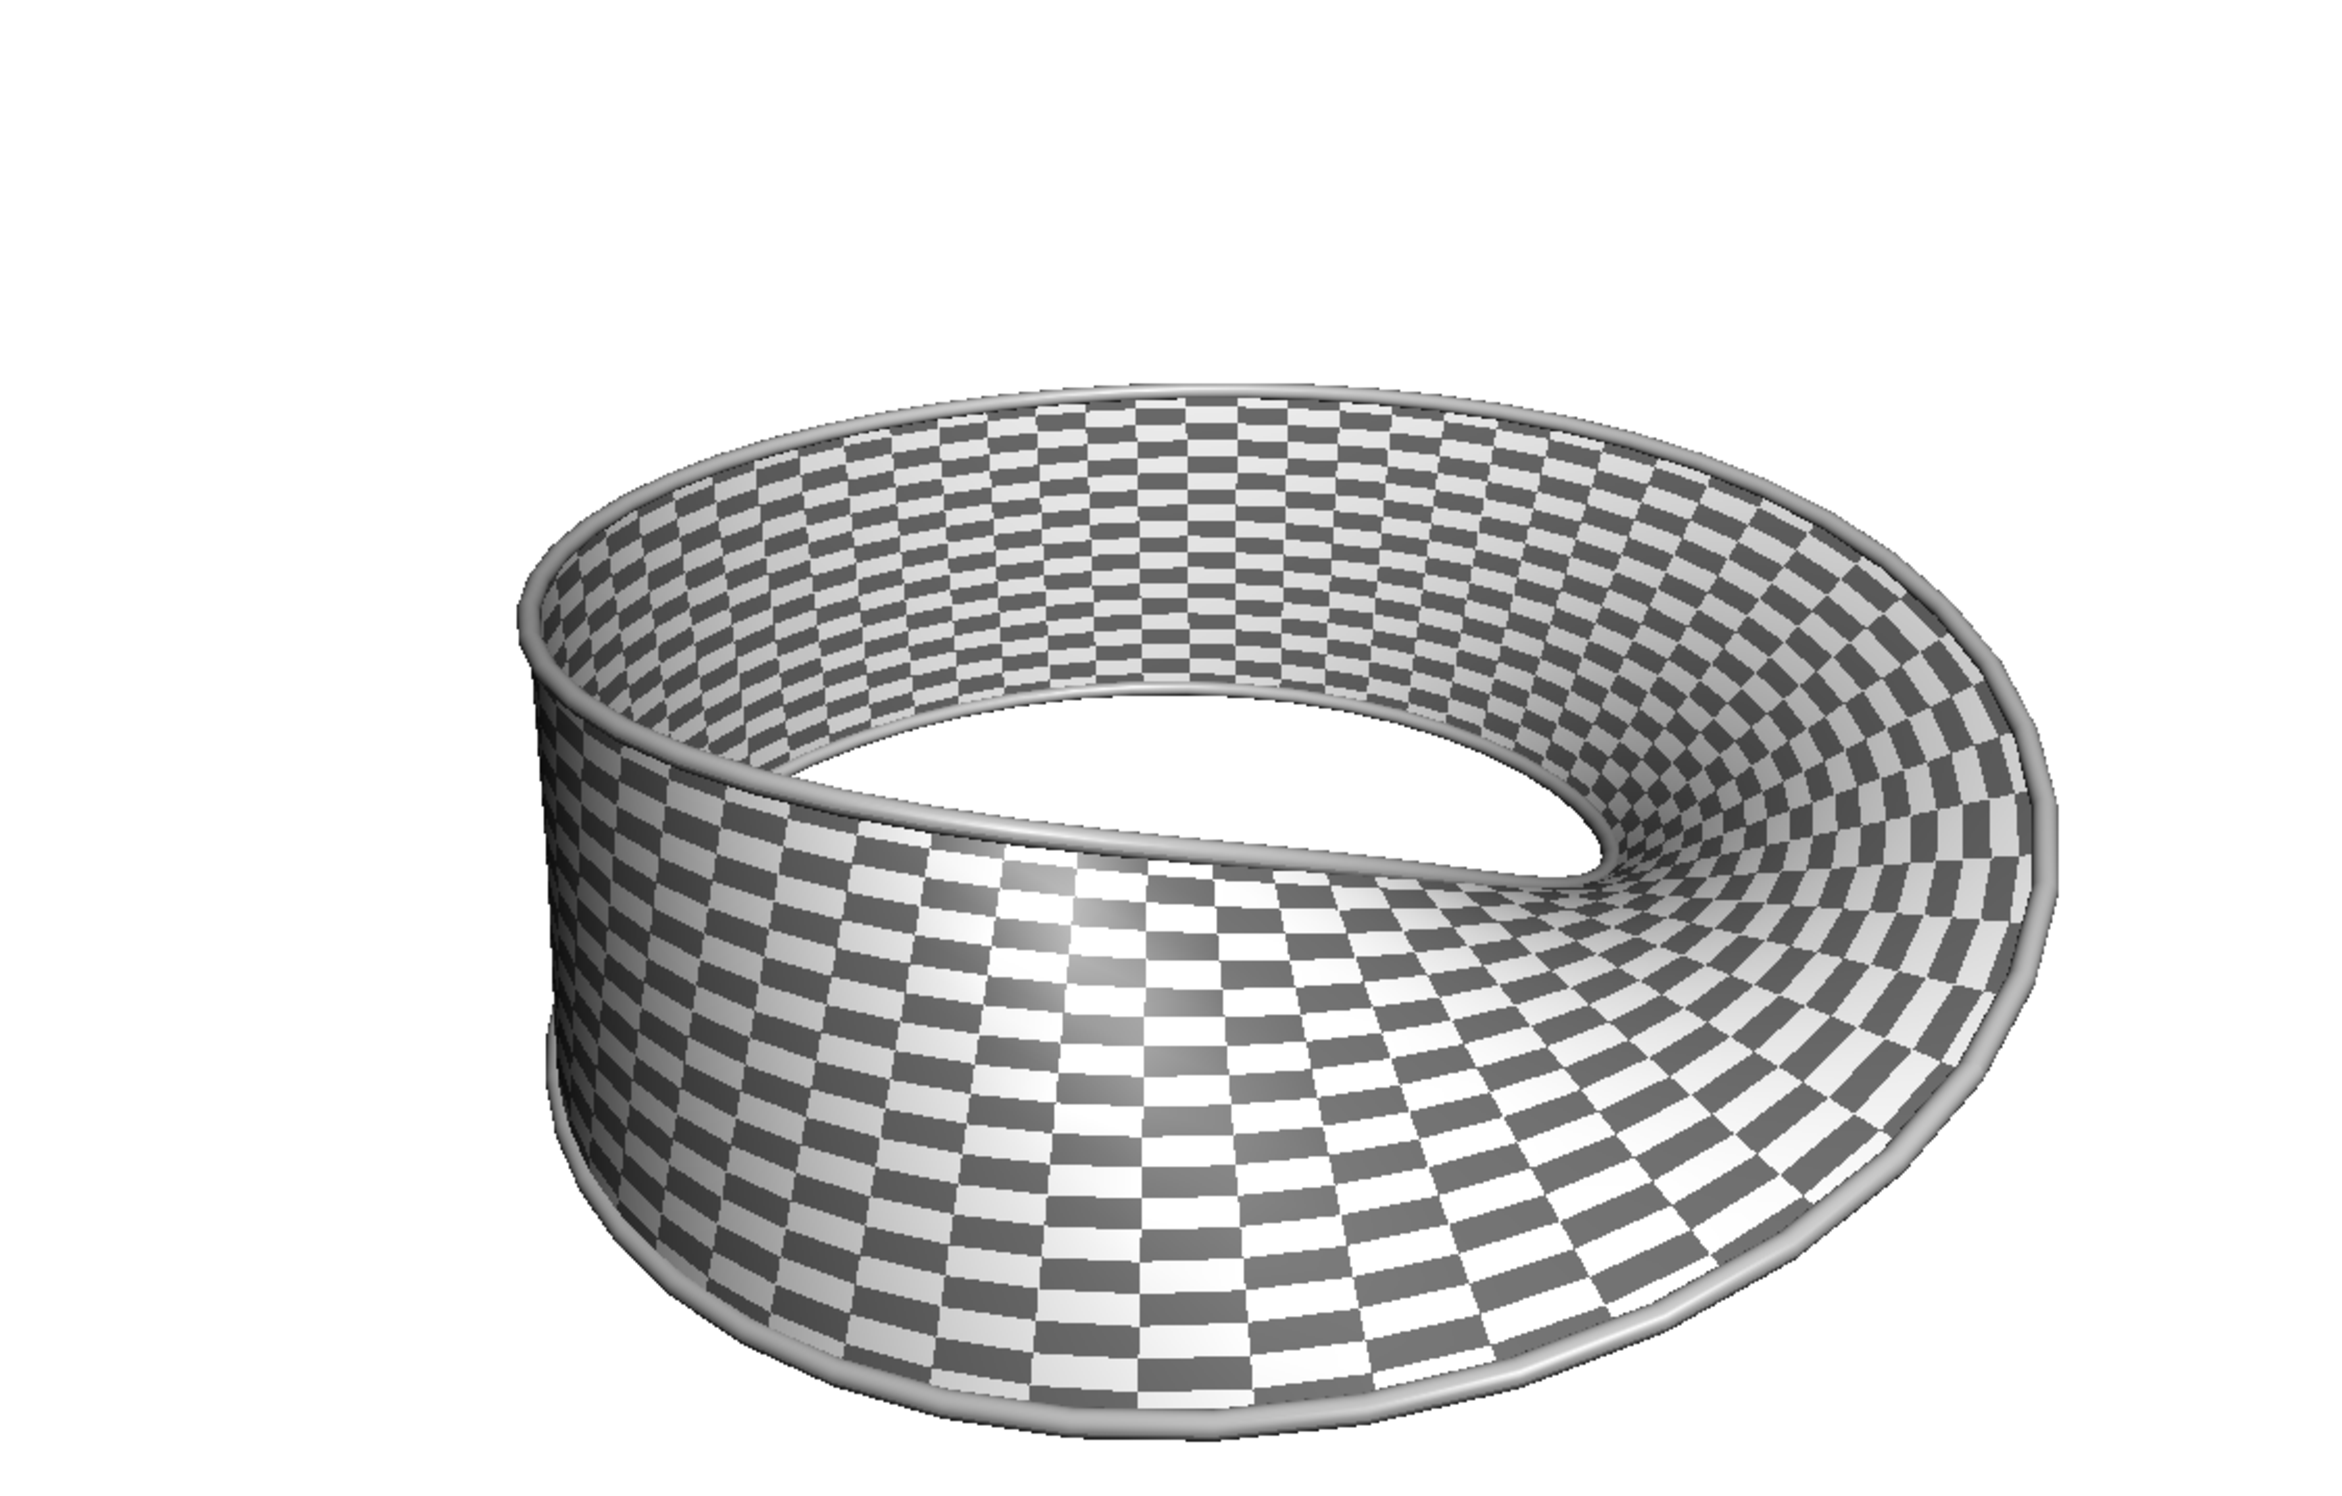
\includegraphics[width=3in]{Mobius_with_patches.pdf}
%\end{center}
\section{Ways of Integrating}
In this chapter we will see several different ways of integrating functions of
several variables.  Before introducing them one by one, we spend this section
reviewing how integration was defined in first semester calculus and outlining
the general features that all different ways of integrating have in common.

\subsection{The one variable integral}
To begin, let us quickly recall how the integral of a function of one variable
is defined.  Given a function $y=f(x)$ and an interval $[a,b]$, we choose a
\emph{partition} of the interval $[a,b]$, which means that
\begin{itemize}
\item we split the interval $[a,b]$ into shorter intervals $[x_0, x_1]$, $[x_1,
  x_2]$, \ldots, $[x_{N-1}, x_N]$, where $a=x_0<x_1<\cdots<x_N=b$,
\item and we choose one \emph{sample point} $\xi_k$ from each interval
  $[x_{k-1}, x_k]$.
\end{itemize}
From these ingredients we compute the \emph{Riemann sum}
\[
R = f(\xi_1) \Delta x_1 + \cdots + f(\xi_N)\Delta x_N = \sum_{k=1}^N f(\xi_k)
\Delta x_k
\]
where $\Delta x_k = x_k - x_{k-1}$ is the length of the $k^{\rm th}$ interval.
\begin{figure}[ht]\noindent
  \begin{minipage}[t]{0.4\textwidth}
    \input ../figures/234/04Riemann1D.tex
  \end{minipage}\hspace{3em}
  \begin{minipage}[t]{0.4\textwidth}
    \input ../figures/234/04Riemann1D-fine.tex
  \end{minipage}
  \caption{Riemann sums for $\int_a^b f(x) dx$ with one partition on the left,
    and a finer partition on the right.  The dashed lines in the figure on the
    left indicate where the sample points $\xi_k$ were chosen.}
  \label{fig:04Riemann1D}
\end{figure}

For most functions $y=f(x)$ it is true that upon making the intervals $[x_{k-1},
x_k]$ shorter (and hence choosing more partition intervals), the resulting
Riemann sums approach a limiting value.  When this happens we call the limiting
value of the Riemann sums \textit{the integral of the function $f(x)$ over the
  interval $[a,b]$}:
\[
\int_a^b f(x) dx = \lim_{%
  \parbox{6em} {\footnotesize\sffamily \centering{``as the partition\\ gets
      finer''}}
} f(\xi_1) \Delta x_1 + \cdots + f(\xi_N)\Delta x_N .
\]
The individual terms in the Riemann sum are areas of the narrow rectangles in
the figure.  Added together they approximate the area of the region under the
graph, so that the integral is the area between the graph of $y=f(x)$ and the
$x$-axis (at least in the case that $f$ is a positive function, so that its
graph lies above the $x$-axis.)

\subsubsection*{A note about rigor}
Our quick description of the single variable integral is lacking in mathematical
precision.  It is based on a belief that we know what ``area'' is.  In the late
19$^{\rm th}$ and early 20$^{\rm th}$ centuries many examples of geometric
figures were found in which area computations give unexpected and
counterintuitive results.  Therefore one cannot base a theory on our intuitive
idea of ``area,'' and instead the integral, defined as limit of Riemann sums is
used a way of giving a rigorous definition of the notion of ``area.''  For a
proper treatment of these issues the student is referred to a more advanced
course on Real Analysis (e.g.~Math 421 or 521).


\subsection{Generalizing the one variable integral}  
While there is essentially only one kind of integral in single variable
calculus, there are many different ways of integrating functions of several
variables.  All these different notions of ``integral'' fit the following broad
description.

In any kind of integral we have these ingredients:
\begin{itemize}
\item a \emph{domain}. Depending on the kind of integral, this can be a region
  in the plane, a region in space, a plane curve, a space curve, or even some
  surface in three dimensional space.
\item a \emph{function} that is defined on the domain
\item a way of measuring the ``\emph{size}'' of pieces of the domain
\end{itemize}
To define the integral we ``partition'' the region, i.e.~we divide it into lots
of little pieces. Given any such partition of the region into smaller pieces, we
then form the following ``Riemann sum''
\[ {\sum_{\parbox{6em}{\footnotesize\sffamily\centering{%
        pieces in the partition}} }}
\Bigl(\parbox{6em}{\footnotesize\sffamily\centering%
  $f$ at sample point\\ in piece \#k} \Bigr) \times \bigl\{\textsf{Size of piece
  \#k}\bigr\}
\]
This gives us a number for each way of partitioning the region.  As we make the
partition finer, i.e.\ as we choose more, smaller, pieces, the Riemann sums tend
to get closer to one particular number, which is called the integral of the
function.  In short, the integral is the limit of the Riemann sums we find as we
take finer and finer partitions:
\[
\lint_{\textsf{some region}} f(x)\; dx =
\lim_{\parbox{4em}{\footnotesize\sffamily\centering{%
      as the\\ partition\\ gets finer}} }
\sum_{\parbox{6em}{\footnotesize\sffamily\centering{%
      pieces in the partition}} }
\Bigl(\parbox{6em}{\footnotesize\sffamily\centering%
  $f$ at sample point\\ in piece \#k} \Bigr) \times \bigl\{\textsf{Size of piece
  \#k}\bigr\}
\]
Depending on what kind of function we have, and what kind of region the function
is defined on, and also how we decide to measure the size of the small pieces in
the partition, this process can lead to many different kinds of integrals.  The
integrals we will meet in this chapter are \emph{double integrals} and \emph{triple
  integrals};  in the next chapter on vector calculus we will also see \emph{line
  integrals} and \emph{surface integrals}.  See Table~\ref{tab:kindsofintegrals}.

\begin{table}[t]\sffamily\color{darkbluegreen}
  \begin{tabular}{lllr} 
    \toprule
    \rule{0pt}{16pt}%
    \parbox{9em}{\centering \bfseries Kind of integral} & 
    \parbox{7em}{\centering \bfseries Domain} & 
    \parbox{9em}{\centering \bfseries Typical piece of partition} & 
    \parbox{9em}{\centering \bfseries Size of piece}\\[2ex] \midrule
    \rule{0pt}{22pt}%
    \parbox{9em}{\centering \itshape ``Good old 221 Integral''\\ $\int_a^b f(x)\; dx$} & 
    \parbox{7em}{\centering interval\\$a\le x\le b$ } & 
    \parbox{9em}{\centering  small subinterval $(x_{k-1}, x_k)$  } & 
    \parbox{9em}{\centering  length of subinterval $\Delta x_k = x_k -
      x_{k-1}$}\\[3ex]\midrule
    \rule{0pt}{16pt}%
    \parbox{9em}{\centering \itshape Multiple integral\\
      $\iint_D f(x, y) dA $}  & 
    \parbox{7em}{\centering region in\\the plane}  & 
    \parbox{9em}{\centering tiny sub domain}   &  
    \parbox{9em}{\centering area $\Delta A$ of\\tiny sub domain} \\[2ex]\midrule
    \rule{0pt}{16pt}%
    \parbox{9em}{\centering \itshape Multiple integral\\
      $\iiint_D f(x, y, z) dV $}  & 
    \parbox{7em}{\centering region\\in space}  & 
    \parbox{9em}{\centering tiny sub domain}   &  
    \parbox{9em}{\centering volume $\Delta V$ of\\tiny sub domain} \\[2ex]\midrule
    \rule{0pt}{16pt}%
    \parbox{9em}{\centering \itshape Line integral\\
      $\int_{\mathcal{C}} f(x, y)\; ds$}  & 
    \parbox{7em}{\centering curve in\\the plane}  &  
    \parbox{9em}{\centering short sub arc\\of the curve}  &   
    \parbox{9em}{\centering length $\Delta s$ of\\the sub arc}\\[2ex]\midrule
    \rule{0pt}{16pt}%
    \parbox{9em}{\centering \itshape Line integral\\
      $\int_{\mathcal{C}} f(x, y, z)\; ds$}  & 
    \parbox{7em}{\centering curve\\in space}  &  
    \parbox{9em}{\centering short sub arc\\of curve}  &   
    \parbox{9em}{\centering length $\Delta s$ of\\the sub arc}\\[2ex]\midrule
    \rule{0pt}{16pt}%
    \parbox{9em}{\centering \itshape Surface integral\\
      $\iint_{\mathcal{S}} f(x, y, z)\; dA $}  & 
    \parbox{7em}{\centering surface\\in space}  &  
    \parbox{9em}{\centering small patch\\on the surface}  &   
    \parbox{9em}{\centering area $\Delta A$ of\\the patch}\\[2ex]\bottomrule
  \end{tabular}
  \smallskip

  \caption{A list of the different kinds of integrals that we will
    encounter in math 234.}
  \label{tab:kindsofintegrals}

\end{table} %}}}


\section{Double Integrals}  

Let $z=f(x, y)$ be a function of two variables defined on some region $D$ in the
plane.  The \emph{double integral of $f$ over $D$} is defined in terms of
Riemann sums, following the general scheme described in the previous section.
To form a Riemann sum we first need a partition of the region $D$ into smaller
regions $D_1$, \ldots, $D_N$, and we need to choose a sample point $(x_k,y_k)$
from each region $D_k$.  If $\Delta A_k$ is the area of region $D_k$, then the
Riemann sum corresponding to the partition $D_1, \cdots, D_N$ and the choice of
sample points $(x_1, y_1)$, \ldots,  $(x_N, y_N)$ is
\begin{equation}
  R = f(x_1, y_1) \Delta A_1 + \cdots + f(x_N, y_N) \Delta A_N 
  = \sum_{k=1}^N f(x_k, y_k)\; \Delta A_k. 
  \label{eq:04doubleintegral-Riemannsum}
\end{equation}
\begin{figure}[b]
  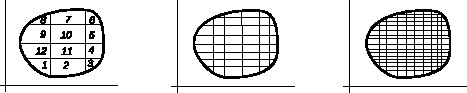
\includegraphics[width=4in]{04refiningapartition-2.pdf}
  \caption{\textbf{On the left: } a region in the plane with some
  partition.
  Many pieces of the partition are rectangles.  This is a common
  choice, but the pieces don't have to be rectangles: here the pieces
  that touch the boundary of the domain have at least one curved edge.
  \textbf{On the right:} the same region with two finer partitions.}
\end{figure}%
If the partition is ``sufficiently fine'' then this Riemann sum will
in many cases be close to one particular number, which we will call
the integral of the function $f$ over the region $D$.  Thus
\begin{equation}
  \liint_{D} f(x,y) \; dA  
  =
  \lim_{\parbox{6em}{\footnotesize\sffamily\centering{%
  as the partition\\ ``gets finer\&finer''}} }\; \;
  \sum_{k=1}^N f(x_k, y_k)\; \Delta A_k. 
  \label{eq:04doubleintegral-defined}
\end{equation}
To make this more precise one has to resort to $\varepsilon$'s and
$\delta$'s, which results in the following definition.

\subsection{Definition}\label{def:04double-integral-eps-delta}\itshape%
If for every $\varepsilon>0$ there is a $\delta>0$ such that the Riemann sum
corresponding to any partition of the region $D$ into smaller pieces $D_1$,
\ldots\,, $D_N$, whose pieces have diameter no more than $\delta$ satisfies
\[
\left|I - \sum_{k=1}^N f(x_k, y_k)\; \Delta A_k\right| <\varepsilon
\]
then we say that
\[
\liint_{D} f(x,y) \; dA  = I.
\]
\upshape

On one hand it can be shown in many cases that that the integral of a function
exists according to the above definition.  On the other hand the
$\varepsilon$-$\delta$ definition is neither a practical method of computing
such integrals, nor does it provide an easy intuitive understanding of the
properties of the integral.  Therefore, we will stick to the less precise
definition \eqref{eq:04doubleintegral-defined} in this course.

\subsection{The integral is the volume under the graph, when $f\ge 0$}
If the function $f$ is positive, then its graph lies above the $xy$-plane, and
there is a simple interpretation of the integral, namely
\[
\liint_{D} f(x, y)\; dA  = \text{\dfnt Volume of }\cR,
\]
where $\cR$ is ``the region under the graph of $f$ above the domain $D$'' -- in
symbols,
\begin{equation}
  \cR = \bigl\{(x, y, z) : (x,y)\text{ lies in }D,\text{ and }
  0\leq z\leq f(x, y)\bigr\}.
  \label{eq:04region-under-graph}
\end{equation}
To see why this is so, imagine that we have a positive function $z=f(x, y)$
defined on some region $D$ in the $xy$-plane, and let us try to compute the
integral $\iint_D f(x, y) dA$ ``geometrically.''
\begin{figure}[t]
  \centering
  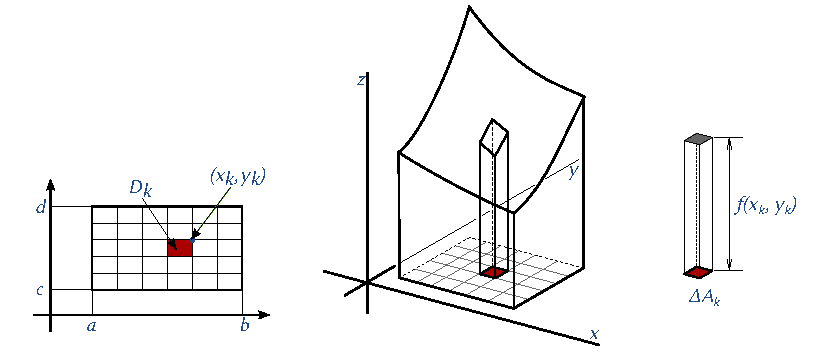
\includegraphics[width=\textwidth]{04Volume-under-graph.pdf}
  \caption{%
    \textbf{On the left: } the domain of the function $f$ partitioned into
    $6\times5$ pieces, each with the same width $\Delta x$ and height $\Delta
    y$.  To form a Riemann sum we have to choose one sample point $(x_k, y_k)$
    in each piece $D_k$ of the partition.  Below we will always choose the
    upper-right-hand corner of the rectangle to be the sample point.  \textbf{On
      the right:} Any piece in the partition corresponds to a term in the
    Riemann sum of the form $f(x_k, y_k)\Delta A_k$. This is the volume of a
    block of height $f(x_k, y_k)$, and base $D_k$, which is approximately the
    volume of the region under the graph of $f$ and above the piece $D_k$.
    Adding all these volumes together we see that a Riemann sum approximates
    the total volume between the graph and the region $D$.}
  \label{fig:04Volume-under-graph}
\end{figure}%
To compute the integral we begin by finely partitioning the region $D$ into
smaller regions $D_1$, $D_2$, \dots, $D_N$ (see
Figure~\ref{fig:04Volume-under-graph} on the left where the small pieces were
themselves chosen to be rectangles).  We also choose one ``sample point'' $(x_k,
y_k)$ in each region $D_k$.  The Riemann sum we get this way is
\[
R = f(x_1, y_1) \Delta A_1 + \cdots + f(x_N, y_N) \Delta A_N
\]
where $\Delta A_k$ is the area of $D_k$.  The $k^{\rm th}$ term, $f(x_k, y_k)
\Delta A_k$, is the volume of a block whose base is $D_k$ and whose top is some
point on the graph of the function above the region $D_k$.  This volume is
almost, but usually not exactly the same as the volume of the region between the
graph of the function and the small region $D_k$ in the $xy$-plane.  The volume
$f(x_k, y_k)\Delta A_k$ of the block above $D_k$ is not exactly the same as the
volume of the region under the graph because the top of the block is a piece of
a horizontal plane while the graph of $f$ will usually have a slope (see
Figure~\ref{fig:04Volume-under-graph}).

The total Riemann sum is therefore the sum of the volumes of such blocks, (see
Figure~\ref{fig:04Riemannsums-for-double-int}) and this will approximate the
volume between the graph of $f$ and the domain of integration $D$.  The finer
the partition, the better the approximation and so we can conclude\footnote{As
  promised before, this is not a very precise ``proof,'' a proof that the limit
  of Riemann sums exists quickly lead us to $\varepsilon$\&$\delta$ arguments.}
that the limit of the Riemann sums is the volume under the graph, i.e.~the
volume of the region $\cR$ defined in \eqref{eq:04region-under-graph}.

\begin{figure}[t]\centering
  \input ../figures/234/04riemannsumcoarse.tex
  \input ../figures/234/04riemannsummedium.tex
  \caption{Approximating the region under the graph of $z=f(x, y)$ from
    Figure~\ref{fig:04Volume-under-graph} by vertical blocks.  The base of each
    block is a rectangle in a partition of the domain of $f$.  As we choose
    finer and finer partitions, the region occupied by the vertical blocks gets
    closer to the region under the graph of $f$.}
  \label{fig:04Riemannsums-for-double-int}
\end{figure}


\subsection{How to compute a double integral}  
\label{sec:how-to-compute-a-double-integral}%
So far, we have a definition for the double integral $\iint_D f(x, y) dA $, and
an interpretation of the integral as ``volume under the graph of $f$.''  What is
missing is a method of actually computing the integral.  In this section we'll
see how one can compute a double integral by doing two one-variable integrals.

Let us take another look at the integral of the function $f$ over the
rectangle
\[
D = \bigl\{(x,y) : a\leq x\leq b, \; c\leq y\leq d\bigr\},
\]
from the previous section.  

We again partition $D$ into smaller rectangles, as in
Figure~\ref{fig:04Volume-under-graph}, but instead of just counting them and
arbitrarily numbering the pieces $1$, $2$, \ldots, $N$, we can use the fact that the
smaller rectangles appear in rows and columns.  If we take $N$ rectangles in the $x$
direction, and $M$ in the $y$ direction, then the smaller rectangles will measure
$\Delta x$ by $\Delta y$, where
\[
\Delta x = \frac{b-a}{N}, \qquad \Delta y = \frac{d-c}{M}.
\]
We let $(x_k, y_l)$ be the upper-right-hand corner of the rectangle in
the $k^{\rm th}$ column from the left, and the $l^{\rm th}$ row from
below.  Then
\begin{equation}
  x_k = a+k \Delta x, \qquad y_l = c+ l \Delta y.
  \label{eq:04xkyl-defined}
\end{equation}
The Riemann sum corresponding to this partition and choice of sample points
$(x_k, y_l)$ is
\begin{equation}
\label{eq:04Doubleint-Riemannsum}
\begin{aligned}
  R\;
  =\;& \sum f(x_k, y_l) \Delta x \Delta y \\  
  =\;& f(x_1, y_1) \Delta x \Delta y \;+\; \cdots \;+\;f(x_{N}, y_1)\Delta x\Delta y +\\
    &f(x_1, y_2) \Delta x \Delta y \;+\; \cdots \;+\;f(x_{N}, y_2)\Delta x \Delta y + \\[-3pt]
    &\hspace{9em}\vdots\\
    &f(x_1, y_{M}) \Delta x \Delta y \;+\; \cdots \;+\;f(x_{N}, y_{M})\Delta x \Delta y
\end{aligned}
\end{equation}
Since we are choosing the upper-right-hand corner of each rectangle as
sample point in that rectangle, the sample point for the rectangle at
the top-right is $(x_{N}, y_{M})$.  (See
Figure~\ref{fig:04Volume-under-graph} on the left.) Therefore, in this
summation $k$ can have any value with $1\le k\le N$ and $l$ can be any
integer with $1\le l\le M$.  


The term corresponding to rectangle $(k,l)$ represents the volume of a
block whose height is $f(x_k, y_l)$ and whose base is a $\Delta
x\times \Delta y$ rectangle.  Together these blocks approximate the
region between the graph of the function and the $xy$-plane.

\begin{figure}[b]
  \input ../figures/234/04riemannsumslicefine.tex
  \caption{
  This picture shows the blocks corresponding to all those terms in
  the Riemann sum $R$ from equation
  \eqref{eq:04Doubleint-Riemannsum} in which $y=y_k$.  These terms $
  \big\{f(x_1, y_k)\Delta x+\cdots+f(x_N, y_k)\Delta x\bigr\}\Delta
  y $ give you the total volume of one row of ``matchsticks'' from
  Figure~\ref{fig:04Riemannsums-for-double-int}.  In this sum $y$ is
  frozen at the value $y=y_k$, so we can think of $f(x_1,
  y_k)\Delta x+\cdots+f(x_N, y_k)\Delta x$ as a Riemann sum for the
  integral $\int_a^b f(x, y_k)\; dx$.}
\end{figure}

Consider the terms on the $k^{\rm th}$ row in
equation~\eqref{eq:04Doubleint-Riemannsum}; after factoring out
$\Delta y$ we get
\[
\text{row \#$k$ of \eqref{eq:04Doubleint-Riemannsum}} = 
\Delta y\; \Bigl\{
f(x_1, y_k) \Delta x + f(x_2, y_k)\Delta x + \cdots + f(x_N, y_k) \Delta x
\Bigr\}.
\]
Note that in this sum the function is always evaluated at the same
value of $y$, namely $y_k$.  The sum between braces $\left\{ \cdots
\right\}$ is actually a Riemann sum for the one-variable integral
\[
I = \int_a^b f(x, y_k) dx
\]
in which we treat $f(x, y_k)$ as a function of $x$ only and consider
the variable $y$ to be frozen at $y=y_k$.
The value of this integral depends on the value at which 
$y$ is frozen, so it is better to write
\[
I(y) = \int_a^b f(x, y) dx.
\]
With this notation we find that 
\[
\text{row \#$k$ of \eqref{eq:04Doubleint-Riemannsum}} 
\approx \Delta y\,\times\,\bigl\{I(y_k)\bigr\} = I(y_k) \Delta y.
\]
To find the value of the Riemann sum that approximates the double
integral $\iint_D f(x,y) dA$ we add the rows in
\eqref{eq:04Doubleint-Riemannsum} and find
\[
R \approx I(y_1)\Delta y+I(y_2) \Delta y + \cdots + I(y_M)\Delta y.
\]
The sum on the right is again a Riemann sum for a one variable
integral, namely, $\int_c^d I(y)dy$.  Therefore we find that 
\[
R\approx \int_c^d I(y) dy 
\]
If we now take the limit in which we let the size of the pieces in the
partition go to zero, then it can be shown (with quite a bit of
effort) that the approximation above gets better, and that one has
\[
\liint_D f(x, y) dA = \int _c^d I(y) dy.
\]
Therefore, remembering the definition of $I(y)$, we have found the
following method of computing a double integral.

\subsection{Theorem} \itshape%  
If $f(x, y)$ is a function defined on a rectangle
\[
D = \left\{ (x,y) : a\leq x\leq b, c\le y\le d \right\},
\]
then the double integral of $f$ over $D$ is given by
\begin{equation}
  \liint_D f(x, y) dA = \int_c^d \Bigl\{\int_a^b f(x, y)
  dx\Bigr\}dy.
  \label{eq:04double-is-iterated-integral-dx-dy}
\end{equation}
One can also first integrate with respect to $y$ and then $x$, so that
\begin{equation}
  \liint_D f(x, y) dA = \int_a^b \Bigl\{\int_c^d f(x, y)
  dy\Bigr\}dx.
  \label{eq:04double-is-iterated-integral-dy-dx}
\end{equation}
\upshape
The second way of computing the double integral $\iint_D f(x, y)\;
dA$, i.e.\ equation \eqref{eq:04double-is-iterated-integral-dy-dx},
follows by the same reasoning that led us to
\eqref{eq:04double-is-iterated-integral-dx-dy}, except in
\eqref{eq:04Doubleint-Riemannsum} one groups the terms by columns
rather than rows.

To compute the right hand side in this equation we have to compute two
one-variable integrals.  The expression
\[
\int_c^d \Bigl\{\int_a^b f(x, y) dx\Bigr\}dy
=\int_c^d \int_a^b f(x, y)\,dx\,dy
\]
is called an \emph{iterated integral}.

The two integrals that appear in an iterated integral are often called ``inner'' and ``outer'' integral:
\[
  \underbrace{\int_c^d
  \Bigl\{
  \underbrace{\color{badgerred}\int_a^b f(x, y) dx}_{\text{inner integral}}
  \Bigr\}
  \;dy}_{\text{outer integral}}.
\]

\subsection{Example: the volume under the graph of  
the paraboloid $z=x^2+y^2$ above the square $Q=\{(x, y) : 0\leq x\leq 1,
0\leq y\le 1\}$}
The double integral we have to compute is
\[
\text{Volume} = \liint_Q \bigl( x^2+y^2 \bigr) dA
\]
and to compute it we write it as an iterated integral
\[
\liint_Q \bigl( x^2+y^2 \bigr) dA = 
\int_0^{1} \Bigr\{ \int_0^1 (x^2+y^2)dx \Bigl\}dy .
\]
In the inner integral the variable $y$ is frozen, so to compute the inner
integral, we simply treat $y$ as a constant, and integrate with respect
to $x$.  We get
\[
\int_0^1 (x^2+y^2)dx  = 
\bigl[\tfrac13x^3 + y^2 x\bigr]_{x=0}^1 =
\tfrac13 + y^2.
\]
(This is $I(y)$ in the notation of the previous section.)

\begin{figure}[ht]
  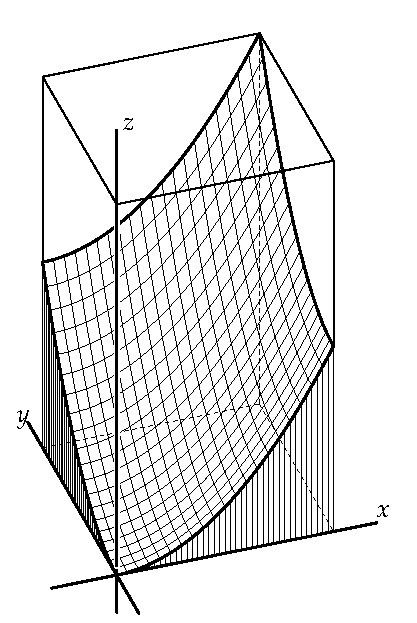
\includegraphics[width=0.4\textwidth]{04Doubleint-example.pdf}
  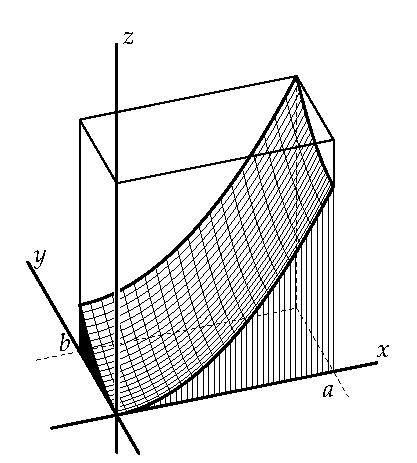
\includegraphics[width=0.4\textwidth]{04Doubleint-example1.pdf}
  \caption{The graph of $z = x^2 + y^2$ above the unit square $Q$ on the
  left, and rectangle $\{ (x, y) : 0\le x\le a$ and $0\le y\le b\}$,
  on the right, together with the surrounding block.  \textit{What
  fraction of the volume of the block lies below the graph?}}
  \label{fig:04Volume-under-graph-examples}
\end{figure}

To get the double integral we must still do the outer integral:
\begin{align*}
  \liint_Q \bigl( x^2+y^2 \bigr) dA
  &= \int_0^{1} \Bigr\{ \int_0^1 (x^2+y^2)dx \Bigl\}dy  \\
  &= \int_0^{1} \bigl(\tfrac 13 +y^2\bigr) dy \\
  &= \bigl[\tfrac 13 y + \tfrac 13 y^3\bigr]_0^{1} \\
  &= \tfrac 13+ \tfrac 1{3} = \tfrac 23.
\end{align*}
Since the surrounding block (Figure
\ref{fig:04Volume-under-graph-examples}) is a $1\times1\times2$ block,
its volume is $2$, and the region under the graph occupies exactly one
third of the whole block.

To compute the volume of the region under the graph of the same
function above the rectangle $\{(x,y) : 0\leq x\leq a, 0\leq y\leq b\}$
one can compute either of the iterated integrals
\[
\int_0^a\int_0^b \bigl(x^2 + y^2\bigr) \; dy\; dx
\text{ or }
\int_0^b\int_0^a \bigl(x^2 + y^2\bigr) \; dx\; dy.
\]

\subsection{Double integrals when the domain is not a rectangle}
\label{sec:04double-integral-not-over-a-block} 
We have seen how to compute a double integral when the domain is a
rectangle.  The reasoning that led us from a double integral to an
iterated integral also works for non rectangular domains, provided
they are not too complicated.  Suppose we want to compute $\iint_D
f(x, y) dA$ where the domain $D$ is the region caught between the
graphs of two functions:
\[
D = \bigl\{(x, y) : a\leq x\leq b, \; f(x)\le y\le g(x)\bigr\}.
\]
We again partition the region by cutting it along many vertical lines
$x=x_1$, $x=x_2$, \ldots, $x=x_N$, and many horizontal lines $y=y_1$,
\ldots, $y=y_M$.  Most of the pieces of the partition will be
rectangles, but those that overlap with the boundary of the region
$D$ may have curved edges.  See
Figures~\ref{fig:04Doubleint-not-a-rectangle} and
\ref{fig:04parabolic-office-building}.

\begin{figure}[htb]
  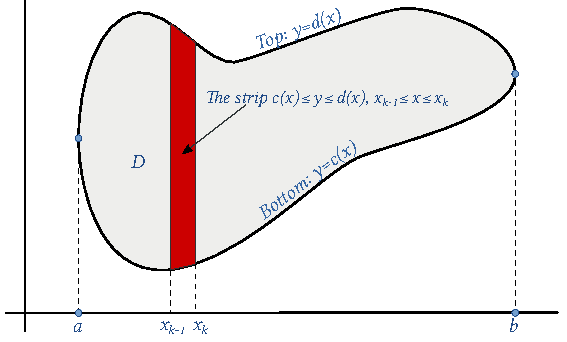
\includegraphics{04Doubleint-not-a-rectangle.pdf}
  \caption{The region between the graphs of $y=f(x)$ and $y=g(x)$.}
  \label{fig:04Doubleint-not-a-rectangle}
\end{figure}

This time, all the terms in a Riemann sum corresponding to one
particular strip $x_{k-1} \le x\le x_k$ add up to a Riemann sum for an
integral over the $y$ variable,
\[
\int_{c(x)}^{d(x)} f(x_k, y)\; dy \; \times \;  \Delta x,
\]
and adding all these we get the iterated integral
\begin{equation}
  \liint_{D} f(x, y) \;  dA 
  = \int_a^b \Bigl\{\int_{c(x)}^{d(x)} f(x, y) \; dy\Bigr\} \; dx.
  \label{eq:04Doubleint-between-two-graphs}
\end{equation}

\subsection{An example--the parabolic office building}  
\label{sec:04parabolic-office-building}
Consider the region under the graph of $f(x, y) = x+y$, above the
domain 
\[
D = \left\{ (x,y) : 0\le x\le 1, (1-x)^2\le y\le 1 \right\}.
\]
The volume of this region is given by
\[
V = \liint_D (x+y)dA.
\]
We can compute this volume by finding the following iterated integral
\begin{equation}
  V = \int_{x=0}^1 \int_{(1-x)^2}^1 (x+y)\; dy\; dx.
  \label{eq:04parabolic-office-building-dy-dx}
\end{equation}
Alternatively, the region $D$ can also be described as
\[
D = \left\{ (x, y) : 0\le y\le 1,\;  1-\sqrt{y} \le x\le 1 \right\}.
\]
This leads to the following iterated integral for the volume
\begin{equation}
  V = \int_{y=0}^1 \int_{1-\surd y}^1 (x+y) \; dx\; dy.
  \label{eq:04parabolic-office-building-dy-dx}
\end{equation}
Both iterated integrals should give the same answer.
\begin{figure}[ht]
  \begin{minipage}[b]{0.4\textwidth}
    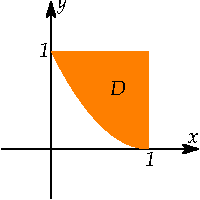
\includegraphics{04Doubleint-example2-domain.pdf}\\
    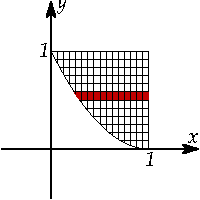
\includegraphics{04Doubleint-example2-partition.pdf}
  \end{minipage}
  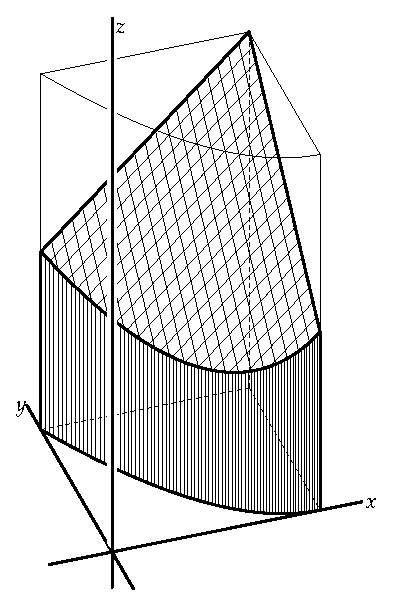
\includegraphics[width=0.5\textwidth]{04Doubleint-example2.pdf}

  \caption{\textbf{On the left: } the domain of integration, a partition, and
  all pieces in the partition corresponding to one value of $y$.
  \textbf{On the right: } The ``parabolic office building,'' being the
  region whose volume is computed in example
  \ref{sec:04parabolic-office-building}}
  \label{fig:04parabolic-office-building}
\end{figure}
Let's compute the first one:
\begin{align*}
  V&= \int_{0}^1 \int_{(1-x)^2}^1 (x+y)\; dy\; dx \\
  &=\int_0^1 \left[ \tfrac12 xy + \tfrac12y^2 \right]_{(1-x)^2}^1\; dx \\
  &=\int_0^1 \left[
                x\bigl(1-(1-x)^2\bigr) +
                  \tfrac12\bigl(1^2-(1-x)^4\bigr)
             \right]\; dx\\
  &=\int_0^1 \left[ 
  2x^2 - x^3 + \tfrac12\bigl(4x-6x^2+4x^3-x^4\bigr)
  \right]\; dx\\
  &=\int_0^1 \left[ 
          2x^2 - x^3 + 2x-3x^2+2x^3-\tfrac12x^4
  \right]\; dx\\
  &= \tfrac23 -\tfrac14 + 1 -1 + 2\times\tfrac14 - \tfrac12 \times\tfrac15\\
  &= \tfrac{16}{15}.
\end{align*}
Note that even though the function we integrated is very simple
(it's just $x+y$) the integral can still become complicated because
of the shape of the domain $D$ over which we are integrating.

\subsection{Double integrals in Polar Coordinates}  
\label{sec:04double-integrals-in-PC}
Sometimes Cartesian coordinates are just not the best choice. 
For instance, a disc or radius $R$, centered at the origin, is very
easy to describe in polar coordinates as ``all points with $r\le R$.''
In Cartesian coordinates we need Pythagoras, and we have to say
``all points with $x^2+y^2\le R^2$.''
\begin{figure}[ht]
  \input ../figures/234/04Polar-partition.tex
  \qquad
  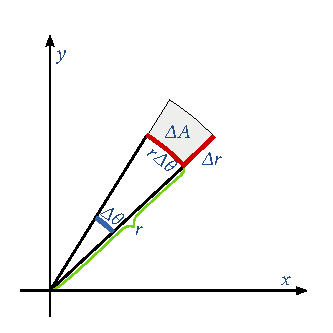
\includegraphics[scale=0.75]{04dAinPC.pdf}
  \caption{\textbf{Left: } A ``polar rectangle'' and a partition by
  lines of constant $\theta$ (the spokes) and curves of constant $r$ (the arcs).
  \textbf{Right: } The area of a small piece of such a partition 
  is approximately $\Delta A \approx \Delta r\times
  r\Delta\theta$.}
  \label{fig:04dAinPC}
\end{figure}
In the same spirit a ``polar rectangle'' is a domain of the form
\[
R = \left\{ \text{all points with }
\theta_0 \le \theta \le \theta_1, r_0 \le r\le r_1
\right\}.
\]
See Figure~\ref{fig:04dAinPC} (on the left).  There is a very natural
way of partitioning such a region into many smaller regions, by
cutting the region along curves of constant $r$ (arcs centered at the
origin) or constant $\theta$ (rays emanating from the origin).
If the partition is sufficiently fine, then the pieces in the
partition will almost be real Cartesian rectangles, with sides
$r\Delta\theta$ and $\Delta r$ ($\Delta\theta$ being the angle between
adjacent rays, and $\Delta r$ being the difference in radius between two
consecutive arcs).  The area of such a small partition piece is
therefore $\Delta A \approx r\Delta\theta\times\Delta r$, and one
arrives at the following formula for the integral of a function of a
polar rectangle
\begin{equation}
  \liint_R f(x, y) \; dA
  =
  \int_{r_0}^{r_1} \int_{\theta_0}^{\theta_1}
  F(r, \theta)\; rd\theta\; dr
  =
  \int_{\theta_0}^{\theta_1} \int_{r_0}^{r_1}
  F(r, \theta)\; rdr\; d\theta.
  \label{eq:04integral-over-polar-rectangle}
\end{equation}
Here $F(r, \theta) = f(r\cos \theta, r\sin\theta)$ is the function
$f(x, y)$ written in polar coordinates.\footnote{It is very common to
use the same letter $f$ for both functions, i.e.\ to write $f(x,y)$
for $f$ as a function of Cartesian coordinates, and also $f(r,
\theta)$ for the same function but written in Polar coordinates.  This
begs the question of what ``$f(0.3, 1.24)$'' means -- are $(0.3, 1.24)$
the Polar or the Cartesian coordinates of the point at which $f$ is to be
evaluated?  To avoid this kind of ambiguity we will try to use different
letters for the same quantity regarded as a function of Cartesian
coordinates, and of Polar coordinates.}

\begin{figure}[h]
  \centering
  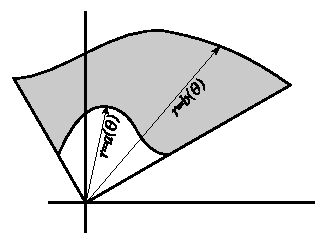
\includegraphics{04polar-domain.pdf}
  \caption{The gray region is the region between the polar graphs
  $r=a(\theta)$ and $r=b(\theta)$.}
  \label{fig:04region-between-polar-graphs}
\end{figure}
There is a similar formula for more complicated domains.
If a domain can be described in polar coordinates by
\[
D = \left\{ \text{all points with } \alpha\le\theta\le\beta, a(x)\leq
r\leq b(x) \right\}
\]
and if we want to integrate a function $z=f(x, y)$ of this domain,
then we can again partition the domain $D$ into many small pieces that are
bounded by circular arcs centered at the origin, and rays emanating
from the origin. The area of a small piece in the partition is once
again given by $\Delta A \approx \Delta r\times r\Delta\theta$, and
therefore the integral of $f$ over $D$ is
\begin{equation}
  \liint_D f(x, y)\;  dA
  =
  \int_\alpha^\beta \int_{a(\theta)}^{b(\theta)}
  F(r, \theta) \; r\; dr\; d\theta.
  \label{eq:04integral-between-polar-graphs}
\end{equation}
\begin{figure}
  \begin{picture} (240.000000,240.000000)(0,0)
    \put(0.0, 0.0){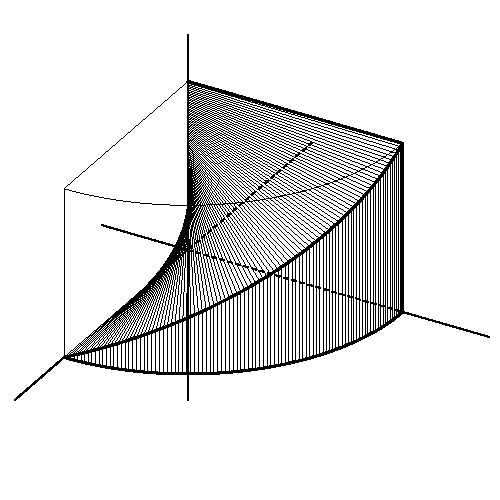
\includegraphics{04under-the-helix.pdf}}
        \put(  6.95,  39.86){\sffamily\itshape $x$}
    \put(226.53,  70.35){\sffamily\itshape $y$}
    \put( 93.25, 219.06){\sffamily\itshape \makebox[0pt][l]{$z$}}
    \put( 83.25, 200.94){\sffamily\itshape \makebox[0pt][r]{$\pi/4$}}

\end{picture}

  \caption{The graph of the function $z=a\theta$ in polar coordinates is called the
  \textit{helicoid}.   Here we see one quarter turn of a helicoid with $a=\frac12$.
  The volume under the helicoid is given by a double integral which is best computed
  using polar coordinates.  \itshape Which fraction of the volume in the surrounding
  quarter cylinder lies beneath the helicoid?  }
  \label{fig:04under-the-helix}
\end{figure}

\subsection{Example: the volume under a quarter turn of a helicoid}
A \emph{helicoid} is the surface that in polar coordinates is
given by 
\[
z=a\theta
\]
where $a>0$ is some constant.  (See Chapter~III, \S~\ref{sec:functions-in-PC-theta})

If we choose the constant $a=\tfrac12$, and take the first quarter turn of this surface, on which $0\le \theta \le \tfrac12\pi$, then we get the picture in Figure~\ref{fig:04under-the-helix}.
In that drawing we have only included the part with $0\leq r\leq 1$.
To compute the volume of the region under the quarter helicoid using
Cartesian coordinates, we would have to compute this integral
\[
V = \int_0^1 \int_0^{\sqrt{1-x^2}} \tfrac12\arctan\frac yx\; dy\; dx.
\]
(Try to set up this integral yourself!)

In Polar coordinates things are easier.  The domain is a polar rectangle, 
\[
0\le r\le 1, \quad 0\le \theta \le \tfrac12\pi,
\]
and the function is very simple,
\[
F(r, \theta) = \tfrac12 \theta.
\]
The double integral that represents the volume is therefore
\begin{equation*}
  V  = \liint_D \tfrac12\theta \; dA 
  = \int_0^1 \int_0^{\pi/2} \tfrac12 \theta r\; d\theta\; dr 
  = \frac{\pi^2}{32}.
\end{equation*}


\section{Problems} 

\problemfont\noindent
\begin{minipage}{0.44\textwidth}
\problem Compute these iterated integrals: 

\subprob $\DS \int_0^1 \int_0^4 x\;  dy\;  dx$ 
\answer %%%%%%%%%%%%%%%%%%%%%%%%%%%%%%%%%%%%%%%%%%%%%%%%%
$2$
\endanswer

\subprob $\DS \int_0^1 \int_0^4 x \; dx\;  dy$ 
\answer %%%%%%%%%%%%%%%%%%%%%%%%%%%%%%%%%%%%%%%%%%%%%%%%%
$8$
\endanswer 

\subprob $\DS \int_{-1}^1 \int_0^{x^2} \; dy \; dx$ 
\answer
$2/3$
\endanswer
\end{minipage}\hfill
\begin{minipage}{0.44\textwidth}
\subprob $\DS \int_0^\pi \int _0^y \frac{\sin y}{y}\; dx\; dy$ 
\answer
$\DS \int_0^\pi \int _0^y \frac{\sin y}{y}\; dx\; dy
=
\int_0^\pi \frac{\sin y}{y} \cdot y \; dy = \int_0^\pi \sin y \; dy =
2$.
\endanswer

\subprob $\DS \int_0^\pi \int _0^\theta \frac{\sin \theta}{\theta}\;dr\; d\theta$ 
\answer
Except for a change in notation ($y\to\theta$ and $x\to r$) this is
the same integral as in the previous problem.  The answer is again $2$.
\endanswer

\subprob $\DS \int_0^1 \int _0^{\sqrt{1-x^2}}\; dy\; dx$ 
\answer
Which function is being integrated?  It's the function $f(x, y) = 1$.

\noindent
$\int_0^1 \int _0^{\sqrt{1-x^2}}\; dy\; dx
=\int_0^1 \bigl[y\bigr]_{y=0}^{y=\sqrt{1-x^2}}\; dx
= \int_0^1 \sqrt{1-x^2}\; dx$.
The last integral
is the area of a quarter circle with radius 1, so the answer is $\pi/4$.
\endanswer
\end{minipage}

\problem What is wrong with the iterated integral 
\[
\int_x^1 \Bigl\{\int_0^1 \sin(\pi x) dx \Bigr\}dy\quad ?
\] 
Is the answer a number -- does it depend on $x$ or $y$?
\answer
Once you compute the inner integral
\[
\int_0^1 \sin(\pi x) dx  = \left[ -\frac1\pi\cos\pi x \right]_{x=0}^1
=-\frac1\pi\cos \pi - \frac1\pi (-\cos 0) = \frac 2\pi,
\]
you get 
\[
\int_x^1 \Bigl\{\int_0^1 \sin(\pi x) dx \Bigr\}dy
=\int_x^1 \frac 2\pi dy = \left[ \frac 2\pi y \right]_{y=x}^1 = \frac 2\pi (1-x).
\]
The result depends on $x$.  The $x$ in the answer and the two $x$-es
in the inner integral refer to different quantities.  This is at best
confusing, and should really never be done.
\endanswer

\problem 
\subprob Is the following true or false? 
  \textit{For any two functions $f(x)$ and $g(y)$ one has}
\[
\int_0^1 \int_0^2 f(x) g(y) \; dx\; dy
= 
\left(\int_0^1 f(x) \; dx\right)
\; \cdot\; 
\left(\int_0^2 g(y)\; dy\right)
\; .
\]
Explain your answer  (if you claim ``true'' give a proof, if you claim ``false'' give
a counterexample.)
\answer
Not true!
To give a counterexample for the statement in the problem, almost any
two functions $f$ and $g$ will do.  For instance, if you choose $f(x) = x$, $g(y)=1$, then you get
\[
\int_0^1 \int_0^2 f(x) g(y) \; dx\; dy= \int_0^1\int_0^2 xdx dy = 2.
\]
but
\[
\int_0^1 f(x) \; dx\; \times\; 
\int_0^2 g(y)\; dy
=
\int_0^1 x \; dx\; \times\; 
\int_0^2  dy
=
\frac{1}{2}\times2 = 1.
\]
\endanswer

\subprob Is the following true or false? 
  \textit{For any two functions $f(x)$ and $g(y)$ one has}
\[
\int_0^2 \int_0^1 f(x) g(y) \; dy\; dx
= 
\left(\int_0^1 f(x) \; dx\right)
\; \cdot\; 
\left(\int_0^2 g(y)\; dy\right)
\; .
\]
Explain your answer (no, this is not the same question as before.  Look at the
integration bounds.) 
\answer
True!
\[
  \int_0^1\int_0^2 f(x)g(y) dy dx
  =\int_0^1\left\{ \int_0^2 f(x)g(y) dy \right\}dx .
\]
Since $f(x)$ does not depend on $y$, we have
\[
\int_0^2 f(x)g(y) dy=f(x) \int_0^2 g(y)\, dy.
\]
Therefore 
\[
  \int_0^1\left\{ \int_0^2 f(x)g(y) dy \right\}dx 
  =\int_0^1 f(x) \left\{\int_0^2 g(y) dy \right\}dx .
\]
The integral $\int_0^2 g(y)dy$ is a constant, and does therefore not depend on $x$,
so we can factor it out of the $x$-integral:
\[
  \int_0^1 f(x) \left\{\int_0^2 g(y) dy \right\}dx
  = \int_0^1 f(x)\, dx \cdot \int_0^2 g(y)\, dy,
\]
which is what we had to show.
\endanswer

\subprob Suppose $D$ is the unit disc, $D=\{(x,y): x^2+y^2<1\}$.  True or False:
\textit{For any two functions $f(x)$ and $g(y)$ one has}
\[
\iint_ D f(x) g(y) \; dx\; dy
= 
\left(\int_{-1}^1 f(x) \; dx\right)
\; \cdot\; 
\left(\int_{-1}^1 g(y)\; dy\right)
\; .
\]
Again, explain your answer.
\answer
This is false, and there is no simple way of fixing it.  To see that this fails
evaluate both sides with $f(x) = 1$ and $g(y)$.  On the left you get the area of
the disc $D$, which is $\pi$, and on the right you get $2\cdot2=4$.
\endanswer


\problem Answer the question posed in
Figure~\ref{fig:04Volume-under-graph-examples}.
\answer
The volume under the graph is
$\frac13 ba^3 + \frac13 ab^3 = \frac 13 ab(a^2+b^2)$.
The volume of the surrounding block is $a\times b\times (a^2+b^2)$, so
the region beneath the graph occupies one third of the surrounding
block, no matter which $a$ or $b$ you choose.
\endanswer


\problem Compute the following double integrals.  
In each case sketch the domain of integration and
show which iterated integral you must compute to find the given double
integral.

\noindent\parbox{0.8\textwidth}{%
\subprob $\DS \iint_D (1+x) \,dA $
\hfill$D = \left\{ (x,y) : 0\leq x\leq 2, 0\leq y\leq 4 \right\}$.
}
\answer
$16$
\endanswer

\noindent\parbox{0.8\textwidth}{%
\subprob $\DS \iint_D (x+y)\,dA $ 
\hfill$D = \left\{ (x,y) : |x|\leq1, 0\leq y\leq 4 \right\}$.
}
\answer
$4$
\endanswer


\noindent\parbox{0.8\textwidth}{%
\subprob $\DS \iint_D xy \,dA $ 
\hfill$D = \left\{ (x,y) : 0\le x\le y, 1\le y \le 2 \right\}$.
}
\answer
$15/8$
\endanswer


\noindent\parbox{0.8\textwidth}{%
\subprob $\DS \iint_{D} \,dA $ 
\hfill$D = \left\{ (x,y) : \tfrac12y^2\le x\le \sqrt{y}, 0\le y\le 1 \right\}$.
}
\answer
$1/2$
\endanswer


\noindent\parbox{0.8\textwidth}{%
\subprob $\DS \iint_{D} {x^2\over y^2}\,dA $ 
\hfill$D = \left\{ (x,y) : 1\le x\le2, 1\le y\le x \right\}$.
}
\answer
$5/6$
\endanswer


\noindent\parbox{0.8\textwidth}{%
\subprob $\DS \iint_D {y\over e^x}\,dA $ 
\hfill$D = \left\{ (x,y) : 0\le x\le1, 0\le y\le x^2 \right\}$.
}
\answer
$12-65/(2e)$.
\endanswer


\noindent\parbox{0.8\textwidth}{%
\subprob $\DS \iint_D x\cos y\,dA $ 
\hfill$D = \left\{ (x,y) : 0\le x\le \sqrt{\pi/2}, 0\le y\le x^2 \right\}$.
}
\answer
$1/2$
\endanswer


\noindent\parbox{0.8\textwidth}{%
\subprob  $\DS \iint_D  
\sqrt{x^3+1}\,dA $
\hfill$D = \left\{ (x,y) : 0\le y\le 1, \surd y\le x\le 1 \right\}$.
}
\answer
$(2/9)2^{3/2}-(2/9)$
\endanswer

\noindent\parbox{0.8\textwidth}{%
\subprob $\DS \iint_D   y\sin(x^2)\,dA $
\hfill$D = \left\{ (x,y) : 0\le y\le 1, y^2\le x\le 1 \right\}$.
}
\answer
$(1-\cos(1))/4$
\endanswer

\noindent\parbox{0.8\textwidth}{%
\subprob $\DS \iint_D x\sqrt{1+y^2}\,dA $ 
\hfill$D = \left\{ (x,y) : 0\le x\le1, x^2\le y\le1 \right\}$.
}
\answer
$(2\sqrt2-1)/6$
\endanswer

\noindent\parbox{0.8\textwidth}{%
\subprob $\DS \iint_D {2\over\sqrt{1-x^2}}\,dA $ 
\hfill$D$ is the triangle bounded by the $y$ axis, the line $y=1$ and
the line $y=x$.
}
\answer
$\pi-2$
\endanswer

\problem Find the volumes of the following regions 
by computing a double integral.

\subprob the region bounded by $z=x^2+y^2$ and $z=4$. 
\answer
$8\pi$
\endanswer


\subprob the region in the first octant 
bounded by $y^2=4-x$ and $y=2z$.
\answer
$2$
\endanswer


\subprob the region in the first octant 
bounded by $y^2=4x$, $2x+y=4$, $z=y$,
and $y=0$.
\answer
$5/3$
\endanswer

\subprob the region in the first octant 
bounded by\\
$x+y+z=9$, $2x+3y=18$, and $x+3y=9$.
\answer
$81/2$
\endanswer

\subprob the region in the first octant 
bounded by $x^2+y^2=a^2$ and $z=x+y$.
\answer
$2a^3/3$
\endanswer

\subprob the region bounded by $x^2+y^2=4z$ and $z=2$. 
\answer
$8\pi$
\endanswer

\subprob Describe the plane region $\cR$ defined by $x^2+y^2 \leq y$ in polar coordinates, and compute the volume of the three dimensional region that lies above $\cR$ and between the graphs of $z=x^2+y^2$ and $z=y$.
\answer
On the region $\cR$ we have $y\geq x^2+y^2 \geq0$, so in particular, we have $y\geq0$, and therefore  $\cR$ lies above the $x$-axis.
To write $\cR$ in polar coordinates, you set $x=r\cos\theta$, $y=r\sin\theta$.  Then
\[
x^2+y^2 \leq y \iff r^2 \leq r\sin\theta \iff r\leq \sin\theta.
\]
In P.C.~the region is therefore given by
\[
0\leq\theta\leq \pi, \text{ and }0\leq r\leq \sin\theta.
\]
The volume of the region above $\cR$ is
\[
V = \iint\limits_\cR \bigl\{y - (x^2+y^2)\bigr\} dA
=\int\limits_{\theta=0}^\pi \int\limits_{r=0}^{\sin\theta}
\bigl\{r\sin\theta - r^2\bigr\} r\, dr\, d\theta.
\]
The result is $\pi/32$.
\endanswer

\begin{multicols}{2}
\problem The average value of a function $f(x, y)$
over a domain $D$ is by definition
\[
\text{average $f$ over $D$}
=
\frac{\iint_D f(x, y) \;  dA}{\text{area of }D}
\]
Find the average value of $f(x,y)=e^y\sqrt{x+e^y}$ on the rectangle
with vertices $(0,0)$, $(4,0)$, $(4,1)$ and $(0,1)$.

\problem Suppose $f(x)$ is a positive function defined on an interval 
$a\le x\le b$.  
Let $A$ be the area under the graph of $y=f(x)$, ($a\le c\le b$), and
let $B$ be the area under the graph of $y=f(x)^2$ ($a\le c\le b$)

\subprob Compute $\int_a^b \int_0^{f(x)} dy dx$. 
\answer
$A$
\endanswer
\subprob Compute $\int_a^b \int_0^{f(x)} ydy dx$. 
\answer
$B/2$
\endanswer

\problem Let $V$ be the volume under the graph of the function 
\[
z=\frac{2xy}{x^2+y^2},
\]
above the region 
\[
D = \left\{ (x, y) : x\ge0,\;  y\ge0,\; x^2+y^2\le1 \right\}.
\]

\subprob Write an iterated integral for the volume $V$, using 
Cartesian coordinates.  (You don't have to compute the integral you
get.)
\answer
$\DS\int_0^1 \int_0^{\sqrt{1-x^2}} \frac{2xy}{x^2+y^2}\; dy\; dx$.
\endanswer
\subprob Compute $V$ using polar coordinates. 
\answer
In P.C.\ the function simplifies to $F(r,\theta) = 2\sin \theta\cos
\theta$, so the volume is
\[
V = \int_0^1 \int_0^{\pi/2} 2\sin\theta\cos\theta r\; d\theta\; dr
=\int_0^1 \left[ \sin^2\theta \right]_0^{\pi/2} r\; dr
=\tfrac12.
\]
\endanswer

\problem  Let $V$ be the volume 
under the graph of $z=xy$ above the domain
\[
D = \left\{ (x, y) : x\ge0,\;  y\ge0,\; x^2+y^2\le 4 \right\}.
\]
Try to draw the region $D$, and the graph of $z=xy$ above $D$.

\subprob Use Cartesian coordinates to compute $V$. 
(Hint: this is similar to part \textsf{(i)} of the previous problem,
but the integral in this problem isn't as bad.)

\subprob Use Polar Coordinates to compute $V$.  
\end{multicols}
\noproblemfont


\section{Triple integrals}  
Instead of integrating over two-dimensional regions in the plane, we
can also integrate over three-dimensional regions in space.  In this
section we will see the definition, how to compute triple integrals
using iterated integrals, and some examples of how triple integrals
come up in the real world.

\subsection{Definition, and how to compute triple integrals}  
The definition of triple integrals follows the same pattern as that of
double integrals.
Let $D$ be some three dimensional region in three dimensional space:
$D$ could be a cube, a ``block,'' a cylinder, a sphere, or in general,
the region enclosed by some surface.  A particular case is that of a
\emph{rectangular block,} which is a region defined by the inequalities
\begin{equation}
    a_x\le x\le b_x,\quad
    a_y\le y\le b_y,\quad
    a_z\le z\le b_z.
    \label{eq:04rectangular-block}
\end{equation}
To define the triple integral of a function $w=f(x, y, z)$ over such a
region we consider a partition of $D$ into many smaller pieces.
We number the pieces $1, 2, \cdots, N$ and for each $j$ we
choose a sample point $(x_j, y_j, z_j)$ from the $j^{\rm th}$
partition piece.  Let $\Delta V_j$ be the volume of the $j^{\rm th}$
partition piece and consider the Riemann sum
\[
f(x_1, y_1, z_1) \Delta V_1 + \cdots
+ f(x_N, y_N, z_N) \Delta V_N 
= \sum_{j=1} ^N f(x_j, y_j, z_j) \Delta V_j.
\]
If these Riemann sums converge to some number as we choose finer and
finer partitions, then we call this limit is called the \emph{triple
integral, or volume integral, of $f$ over $D$}.  The notation we use is
\begin{equation}
    \liiint_D f(x, y, z) \; dV 
    = 
    \lim_{
    \parbox{4em}{\footnotesize\sffamily\centering
                 {as the\\ partition\\ gets finer}
                }
    }
    \sum_{j=1} ^N f(x_j, y_j, z_j) \Delta V_j.
    \label{eq:04tripleintegral-defined}
\end{equation}
If the domain $D$ is a rectangular block, defined by the inequalities
\eqref{eq:04rectangular-block}, then the triple integral can be
computed by an iterated integral
\begin{equation}
\label{eq:04triple-iterated-integral-over-block}
\liiint_D f(x, y, z) \; dV  
=
\int_{a_z}^{b_z}
\int_{a_y}^{b_y}
\int_{a_x}^{b_x} 
f(x, y, z) \; dx\; dy\; dz.
\end{equation}
This follows from the same kind of arguments that allowed us to turn
a double integral into an iterated integral in
\S~\ref{sec:how-to-compute-a-double-integral}.

We can use \eqref{eq:04triple-iterated-integral-over-block} to compute a triple integral over any three dimensional block.  To compute triple integrals over more general domains we can use the same slicing method as in \S~\ref{sec:04double-integral-not-over-a-block}.
If the domain $D$ is given by inequalities of the type
\begin{equation}\label{eq:04general-domain-3D}
  a_x(y,z)\le x\le b_x(y,z),\quad
  a_y(z)\le y\le b_y(z),\quad
  a_z\le z\le b_z.
\end{equation}
where $a_y(z), b_y(z), a_z(y,z)$, and $b_z(y,z)$ now are functions
rather than constants, then the triple integral of a function
$f(x, y, z)$ over $D$ is given by
\[
\liiint_D f(x, y, z) \; dV  
=
\int_{a_z}^{b_z} 
\int_{a_y(z)}^{b_y(z)} 
\int_{a_x(y,z)}^{b_x(y,z)} 
f(x, y, z) \; dx\; dy\; dz.
\]


\subsection{Example -- the integral of $f(x, y, z)=x^2+y^2$ over  
a rectangular block}\label{sec:04int-of-x2y2-over-block}
Let's compute the integral of $f(x, y, z) = x^2+y^2$ over the domain 
\[
D = \left\{ (x,y,z) : 0\le x\le A,\;  0\le y\le B,\;  0\le z\le C \right\},
\]
where $A$, $B$, and $C$ are the sides of the block.

The integral of $f$ over $D$ is
\[
\liiint_D \bigl(x^2+y^2\bigr)\;  dV
= \int_0^C  \int_0^B  \int_0^A  \bigl(x^2+y^2\bigr)\;  dx\; dy\; dz
\]
It is a good idea to write such an integral as
\[
\liiint_D \bigl(x^2+y^2\bigr)\;  dV
= \int\limits_{z=0}^C  
\int\limits_{y=0}^B  \int\limits_{x=0}^A
\bigl(x^2+y^2\bigr)\;  dx\; dy\; dz
= \tfrac13 ABC \bigl(A^2 + B^2\bigr),
\]
to emphasize which integral goes with which variable.

The computation goes in three steps (there are three integrals).
The innermost integral is
\[
 \int_0^A (x^2+y^2)\, dx
 =
 \tfrac13 A^3 + y^2A.
\]
Next we integrate this with respect to $y$:
\[
  \int_0^B  \int_0^A  \bigl(x^2+y^2\bigr)\;  dx\; dy
  =\int_0^B \bigl(\tfrac13A^3 + y^2A\bigr)\; dy
  = \tfrac13 A^3B + \tfrac13 AB^3.
\]
finally, we integrate with respect to $z$:
\begin{align*}
  \int_0^C  \int_0^B  \int_0^A  \bigl(x^2+y^2\bigr)\;  dx\; dy\; dz
  &=\int_0^C \bigl(\tfrac13 A^3B + \tfrac13 AB^3\bigr) \; dz \\
  &=\tfrac13A^3BC+\tfrac13AB^3C\\
  &= \tfrac13 ABC \bigl(A^2 + B^2\bigr).
\end{align*}

\subsection{Example of setting up a triple iterated integral-- the integral of $e^x$ over the unit sphere}  
Suppose we needed to know the integral
\[
\liiint_D e^x \; dV,
\]
where the domain
\[
D = \left\{ (x,y,z) : x^2+y^2+z^2 \le 1 \right\}
\]
is the unit sphere.
\begin{figure}[t]
  \begin{picture} (200.000000,226.400000)(0,0)
    \put(0.0, 0.0){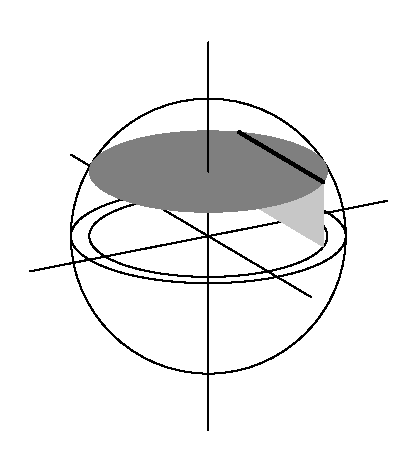
\includegraphics{04integral-over-sphere.pdf}}
        \put(102.00, 206.23){\sffamily\itshape $z$}
    \put(185.74, 133.13){\sffamily\itshape $y$}
    \put(152.50,  83.88){\sffamily\itshape $x$}

\end{picture}

  \caption{\textbf{Turning a triple integral over the unit sphere into
  an iterated integral. } The horizontal gray disc contains all points
  with a given fixed value of $z$; the solid line in that disc
  contains all points at height $z$ whose $y$ coordinate is also fixed
  at a particular value.  From this drawing we can see that $z$ runs
  between $-1$ and $+1$; for any given $z$, the $y$ coordinate runs
  between $-\sqrt{1-z^2}$ and $+\sqrt{1-z^2}$; for fixed $y$ and $z$,
  the $x$ coordinate can take any value between $\sqrt{1-y^2-z^2}$ and
  $\sqrt{1-y^2-z^2}$.}
  \label{fig:04integral-over-sphere}
\end{figure}
By slicing the domain $D$ in the $x$, $y$, and $z$ directions we can describe following the general template in \eqref{eq:04general-domain-3D}:
\begin{itemize}

\item $z$ can take any value between $-1$ and $+1$, 

\item for given $z$ the coordinate $y$ can be anything between $-\sqrt{1-z^2}$ and $+\sqrt{1-z^2}$, 

\item for given $y$ and $z$ the remaining coordinate $x$ can have all values
from $-\sqrt{1-y^2-z^2}$ to $+\sqrt{1 - y^2 - z^2}$.

\end{itemize}
(See Figure~\ref{fig:04integral-over-sphere}.)

This lets us write the triple integral as an iterated integral:
\[
\liiint_D e^x \; dV
=
\int_{-1}^1 \int_{-\sqrt{1-z^2}}^{\sqrt{1-z^2}}
\int_{-\sqrt{1-y^2-z^2}}^{\sqrt{1-y^2-z^2}}
e^z \; dx\; dy\; dz.
\]
Even though it can be computed this is not an easy integral -- the point of
this example was to find the integration bounds in the iterated
integral.

\section{Why compute a Triple Integral?}  

\subsection{The 4D-volume under a graph}  
Just as $\int_a^b f(x)\; dx$ is the area between the graph of the
function $y=f(x)$ and the interval $[a,b]$ on the $x$-axis, and
$\iint_D f(x, y) \; dA$ is the volume caught between the graph of
$z=f(x, y)$ and the domain $D$ in the $xy$ plane, there should be a
similar description of $\iiint_D f(x, y, z)\; dV$.  There is, but it
requires some imagination: 
the graph of $f$ is the set of points in \textit{four
dimensional space} whose coordinates $(x, y, z, w)$ satisfy $w=f(x, y,
z)$, and the triple integral $\iiint_D f(x, y, z) dV$ is the ``four
dimensional volume'' of the four dimensional region caught between
the graph of $f$ and the domain $D$ in $xyz$-space.
Of course, even though people will draw cartoon like representations of
the situation like this,
\begin{figure}[h]\centering
  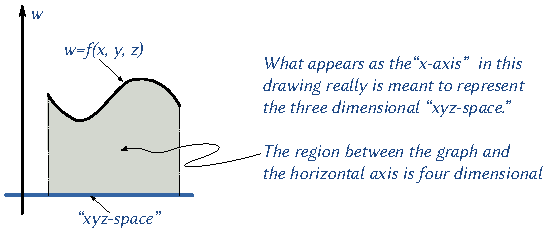
\includegraphics{04-4Dgraph-cartoon.pdf}
\end{figure}\\
we cannot really visualize four dimensional volumes.  Rather than
telling us what the triple integral is, the interpretation
``integral$=$volume'' gives a definition of what
``four dimensional volume'' should be.

\subsection{The average of a function over a domain $D$} 
There is a formula for the ``average value of a function on a region.'' 
The only rigorous definition for the ``average'' is just that formula,
so we could simply state the formula be done with it.  Here it is: the
average of a function $w=f(x,y,z)$ over a region $D$ is defined to be
\begin{equation}
    \parbox{64pt}{\centering\sffamily Average of $f$\\ over $D$ }
    =
    \frac{1}{V_D} \liiint_D f(x, y, z) \; dV.
    \label{eq:04average-defined}
\end{equation}
There is however an intuitive derivation (a story) that justifies why we
call this particular quantity the average.  Understanding this
derivation is at least as important as just knowing the formula
\eqref{eq:04average-defined}.

\subsubsection*{Why \eqref{eq:04average-defined} deserves to be called the average}
What is an average?
If we have finitely many numbers $a_1$, \ldots,\, $a_N$ then their average is
just
\[
\textsf{Average} = \frac{a_1+\cdots+a_N}{N}.
\]
If we only have finitely many points $(x_1,y_1,z_1)$, \ldots \,, $(x_N,
y_N, z_N)$ in the region $D$ then the average function value at these
points is
\[
 \parbox{96pt}{\sffamily\centering Average function value\\ at given points}=
 \frac{f(x_1,y_1,z_1) + \cdots + f(x_N, y_N, z_N)}{N}. 
\]
To define the average of a function over a region $D$, we cannot simply
add all the function values of $f$ at all the points in $D$ because
there are infinitely many such points.  Instead, we sprinkle the region
$D$ with a very large but finite number of points, and calculate the
average value of the function at all these points.  If the points are
evenly distributed, and if there are enough of them, then the average
value of the function at the dots should be a good approximation for the
average value of the function on the region.  E.g.~the average of our
function over the region on the left
\begin{figure}[h]
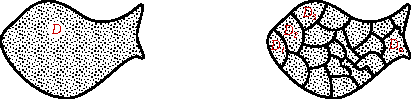
\includegraphics{04average-over-a-fish.pdf}
\end{figure}
should be approximately the average of the function at the dots drawn in that region.

To approximate the average at the dots we partition the region into many
small pieces, which we label $D_1$, \dots, $D_n$.  We write $\Delta V_j$
for the volume of the $j^{\rm th}$ piece $D_j$, and $V_D$ for the volume
of the whole region $D$.  We assume that the pieces are so small that we
may assume that the function is practically constant in each piece.

Since the dots are evenly distributed over $D$, the number of dots in
the $j^{\rm th}$ partition piece is proportional to the volume of that
piece, so
\begin{equation}
 \frac{N_j}{N}
  \approx \frac{\Delta V_j}{V_D} 
\label{eq:number-of-dots-in-Dj}
\end{equation}
where $N_j$ is the number of dots in the $j^{\rm th}$ piece, and $N$ is
the total number of dots.

To compute the average value of $f$ at all the dots we begin with
\[
\text{\sffamily sum of $f$ at all dots}
=\sum_j \text{\sffamily sum of $f$ at all dots in $j^{\rm th}$ piece} \;.
\]
If we pick a sample point $(x_j,y_j,z_j)$ in each piece $D_j$, then,
since the pieces are assumed to be small, we may approximate the
function value at every dot in $D_j$ by the value of the function at the
sample point.  There are $N_j$ dots in $D_j$, so we find that 
\[
\text{\sffamily sum of $f$ at all dots}
\approx \sum_j N_j f(x_j, y_j, z_j)
\]
Using \eqref{eq:number-of-dots-in-Dj} we therefore find that the average
function value at all the dots is
\begin{align*}
  \frac{\text{\sffamily sum of $f$ at all dots}}
       {\text{\sffamily number of dots in $D$}}
  &\approx \frac1N\sum_j N_j f(x_j, y_j, z_j) \\
  &=\sum_j \frac{\Delta V_j}{V_D}f(x_j, y_j, z_j) \\
  &=\frac 1{V_D} \sum_j f(x_j, y_j, z_j)\,\Delta V_j \\
  &\approx \frac1{V_D} \iiint\limits_D f(x,y,z)\, dV.
\end{align*}
This is exactly how we had defined the average of $f$ over the region $D$.

Keep in mind that the above is not a proof of the equation
\eqref{eq:04average-defined}, but rather an intuitive justification for
taking \eqref{eq:04average-defined} as definition of the average.

\subsection{Example \ref{sec:04int-of-x2y2-over-block} continued} 
In \S\ref{sec:04int-of-x2y2-over-block} we computed the volume
integral of
\[
f(x, y, z) = x^2+y^2
\]
over the rectangular block $D$ given by $0\le x\le A$, $0\le y\le B$,
$0\le z\le C$ and we found
\[
\liiint_D \left( x^2+y^2 \right)\; dV = \tfrac13 ABC\bigl(A^2+B^2\bigr).
\]
Since the volume of the block is $ABC$, the average value of
$f(x, y, z) = x^2+y^2$ over the block $D$ is 
\[
    \parbox{96pt}{\centering\sffamily Average of $x^2 + y^2$\\ over $D$ }
=
\frac{\tfrac13 ABC\bigl(A^2+B^2\bigr)}{ABC}
=
\tfrac13 \bigl(A^2 + B^2\bigr).
\]

\subsection{Densities}  
If a substance (for an example, think of a gas in a cylinder) occupies
a certain region $D$ in space, then its \emph{density} $\mu$ is defined to
be 
\[
\mu = \textsf{density} = \frac{\textsf{mass in }D}{\textsf{volume of }D}.
\]
If the substance is evenly distributed throughout the region
$D$, then the mass-to-volume ratio will be the same for any subregion
$D'$.  Thus the mass contained in any smaller region $D'$ will be
proportional to the volume of that region:
\[
\textsf{mass in }D' = \mu \times \textsf{volume of }D'.
\]
When the substance is not distributed evenly this proportionality will
no longer hold, and we say that ``the density varies from point to point.''
If we now want to give a precise definition of \emph{the density at any point}
$P$, we run into the same kind of problem we had in first semester
calculus when we tried to define
the slope of a tangent, or the velocity at one moment in time.  Namely, 
the ``density at $P$'' should be the mass of the substance at $P$ divided
by the volume of the point $P$ -- but there is no mass at one point, and the
volume of one point is zero, so this leads to density$=\frac{0}{0}=$??
The way out of this is to calculate the average density for very small
regions $D'$ surrounding the point $P$, and to declare those as
approximations of the density at $P$.
To get a better approximation we should choose a smaller region $D'$.

This is summarized in the following formula, 
\begin{equation}
  \mu(x, y, z) 
  = 
  \lim_{D'\searrow P}
  \frac{\textsf{mass in }D'}{\textsf{volume of }D'}
  \label{eq:04density-defined}
\end{equation}
where ``$D'\searrow P$'' means that we are taking the limit as the region
$D'$ shrinks to the point $P$.
\begin{figure}[ht]
  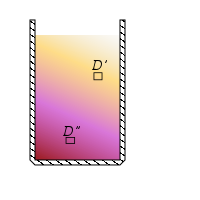
\includegraphics[width=1.7in]{04density.png}
  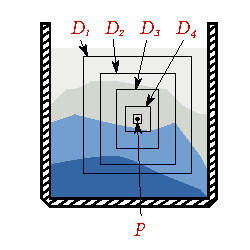
\includegraphics{04defining-density.pdf}
  \caption{
  Density of gas in a container; in these drawings most of the
  gas concentrates in the bottom of the container.
  \textbf{Left: } 
  The total mass in two regions, $D'$ and $D''$, depends on their
  location, even though they have the same shape and volume. 
  \textbf{Right:} To define the density at a point $P$, we compute
  the average density over smaller and smaller regions $D_1$, $D_2$,
  \dots which shrink to the given point $P$.  If the average
  densities converge to some number, then we call that limit the
  density at $P$.}
\end{figure}

\subsection{Mass as integral of the density}  
Suppose the density of a substance is given to us as a function
$\mu(x, y, z)$, how do we find the total mass of the substance present in a
particular region $D$?
The answer is in terms of a triple integral, and the way this integral comes
about is typical for a large number of applications of double and triple
integrals.

To find the total mass present in a region $D$ we partition it into many small
pieces, and compute the mass in each small piece.  Consider one such piece.  If it is
small enough, then we assume that the density $\mu(x, y, z)$ is nearly constant in
that small piece, and hence the total mass in one small piece will be
\[
\textsf{mass in a piece of the partition}
=
\mu(x, y, z) \times \Delta V.
\]
Here $(x, y, z)$ is a sample point in the partition piece, and $\Delta V$
is the volume of the piece.  
So when we compute the total mass by adding all the masses of the
partition pieces, each piece in the partition contributes one term of the
form $f(x, y, z) \Delta V$.  Our formula for the total mass is therefore a
Riemann sum for the following triple integral
\begin{equation}
  \textsf{total mass} 
  =
  \liiint_D \mu(x, y, z)\; dV.
  \label{eq:04totalmass-from-density}
\end{equation}
\subsection{Example: air in the atmosphere.}  
\label{sec:air-in-atmosphere}
\textit{How much air is there in the atmosphere in a vertical column
of height $H$ above one square meter?}

According to one model of the atmosphere, the density of the atmosphere
decays exponentially with height, so that
\begin{equation}
  \mu(x, y, z) = Ce^{-z/L}  \quad ({\rm kg}/{\rm m}^3)
  \label{eq:04air-density}
\end{equation}
\marginpar{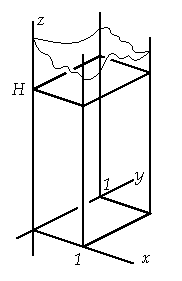
\includegraphics{04air-column.pdf}}
where $z$ is the height above sea level, and $x, y$ are horizontal
coordinates.  The constant $C$ is the density of air at sea level, and
$L$ is another constant ($L$ must have the units of length).

We adapt our coordinates to the $1\times1$ square which is the
base of the air column whose mass we are to compute, namely, we
let the origin be one of the corners of the square, and we let the sides at
this corner be the $x$ and $y$ axes.  The region occupied by 
the air column is then a rectangular block
\[
D = \left\{ (x, y, z) : 0\le x\le 1, 0\le y\le 1, 0\le z\le H \right\}
\]
and the mass of the air in this block is
\begin{align*}
  M &= \liiint_D \mu(x, y, z) \; dV \\
  &= \int_0^H \int_{y=0}^1 \int_{x=0}^1 C e^{-z/L}\; dx\; dy\; dz \\
  &= LC\bigl(1-e^{-H/L}\bigr).
\end{align*}
To get the mass of \textit{all} the air above our $1\times1$ square, we let
$H\to\infty$ which leads to
\[
\textsf{Total Mass} = LC.
\]


\subsection{The moment of inertia of a solid about an axis of rotation} 
\label{sec:moment-of-inertia}
An object of mass $m$ that moves with velocity $v$ has kinetic energy
given by 
\begin{equation}\label{eq:04Kinetic-Energy}
  K=\frac12mv^2.
\end{equation}
If a solid object is rotating about an axis, then it also has kinetic
energy, but the formula \eqref{eq:04Kinetic-Energy} does not apply, because
different parts of the solid will be moving with different velocities.  The
problem is that $v$ is not a constant: it varies from place to place, and
thus it is a function of where we measure the velocity.

\marginpar{\dfnt\centering
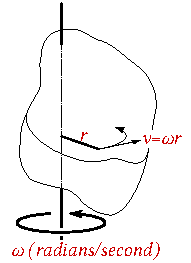
\includegraphics[scale=0.9]{04moment-of-inertia.pdf}\\
the kinetic energy of a whirling potato}
To compute the kinetic energy of a rotating solid we break it up into
small pieces: if each of the pieces is small enough, then all the particles
in that small piece will have nearly the same velocity.  A well known
formula from trigonometry says that if the object is rotating with angular
velocity $\omega$ about an axis, then the velocity of a particle in the
object is given by
\(
v=\omega r
\)
where $r$ is the distance from the particle to the axis of rotation.
On the other hand the mass of such a small piece will be $\mu\cdot\Delta
V$, where $\mu$ is the density of the material (which we assume to be
constant here), and $\Delta V$ is the volume of the small piece.
Therefore if we break the object into many small pieces (partition the
object), the kinetic energy of any one of the small pieces is
\[
\textsf{K.E.~of one piece} = \frac12\mu (\omega r)^2\Delta V.
\]
Adding the kinetic energies of all the small pieces again gives us a
Riemann sum for an integral, and this leads us to the formula
\begin{equation}
  K = \liiint_D \tfrac12\mu\omega^2r^2\; dV
  =\frac12 M\omega^2,
  \label{eq:04kinetic-energy-of-rotating-object}
\end{equation}
where
\begin{equation}
  M \stackrel{\rm def}= \mu\liiint_D r^2 \; dV.
  \label{eq:04moment-of-inertia-defined}
\end{equation}
is called the \emph{moment of inertia} of the given object about the
given axis of rotation.

\subsection{Example}\itshape Compute the moment of inertia of a wooden rectangular block
\[
D = \bigl\{(x, y, z) : 0\le x\le A, 0\le y\le B, 0\le z\le C\bigr\}.
\]
around the $z$ axis. The density of the wood is $\mu$.
\upshape

The integral we have to calculate is 
\[
M = \mu \liiint_D r^2 \; dV.
\]
To compute this we have to figure out what $r$ is: since  $r$ is the
distance from the point $(x, y, z)$ to the axis of rotation, and since this
axis is the $z$-axis, we get, by Pythagoras,
$r^2 = x^2 + y^2$.  Therefore we have to compute
\[
M = \mu \liiint_D \bigl(x^2 + y^2\bigr) \; dV.
\]\marginpar{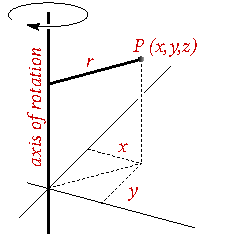
\includegraphics{04distance-to-rotationaxis.pdf}}
We have already computed this integral in
\S\ref{sec:04int-of-x2y2-over-block}, where we found that
\[
M = \tfrac13\mu ABC(A^2+B^2).
\]





\section{Integration in special coordinate systems}  
Many volume integrals arise in situations where there is a lot of
symmetry.  When this happens Cartesian ``$x, y, z$'' coordinates are
usually not the best choice to compute the integral.  There are many
different coordinates besides Cartesian.  In this section we will look
at the two most commonly used coordinate systems.  They can both be
thought of as three-dimensional variations on polar coordinates in the
plane.

\subsection{Cylindrical coordinates}  
Let $P$ be some point in three dimensional space.
If we provide the $z$ coordinate as well as the polar coordinates
$(r, \theta)$ of the projection of $P$ on the $xy$ plane, then the
location of $P$ is completely determined.  See the drawing on the left
in Figure~\ref{fig:04cylindrical-spherical-coords}.  From this drawing
it is easy to derive the relation between cylindrical Cartesian
coordinates
\begin{equation}
  \begin{aligned}
    x &= r\cos \theta \\
    y &= r\sin \theta \\
    z &= z
  \end{aligned}
  \label{eq:04cylindrical-to-cartesian}
\end{equation}

\subsection{Spherical coordinates}  \label{sec:spherical-coordinates}
We can also specify the location of a point $P$ by providing these
three numbers:

-- the distance $\rho$ from $P$ to the origin

-- the angle $\phi$ between the positive $z$-axis and the line from
the origin to the point $P$

-- the polar angle $\theta$ of the projection of $P$ onto the
$xy$-plane.

See the drawing on the right in
\marginpar{\footnotesize\sffamily\color{badgerred}\textbf{DO NOT MEMORIZE.}\\
What if the north pole happens to be on the $x$-axis?  Can you still relate spherical and Cartesian coordinates?
}%
Figure~\ref{fig:04cylindrical-spherical-coords}, from which we can
derive the following relation between the spherical coordinates
$(\rho, \phi, \theta)$ and the Cartesian coordinates $(x, y, z)$ of a
point:
\begin{equation}\label{eq:04spherical-to-cartesian}
  \begin{aligned}
    x &= \rho\sin\phi\cos \theta \\
    y &= \rho\sin\phi\sin \theta \\
    z &= \rho\cos\phi
  \end{aligned}
\end{equation}
The angle $\phi$ takes values between $0$ and $+\pi$, with $\phi=0$ on
the north pole, and $\phi=\pi$ on the south pole.  The polar angle
$\theta$ can take all values from $0$ to $2\pi$, or more generally any
value in some interval of length $2\pi$ (like $-\pi<\theta<\pi$).


\begin{figure}[t]\centering
  \hspace{0.1\textwidth}
  \begin{picture} (120.000000,124.068966)(0,0)
    \put(0.0, 0.0){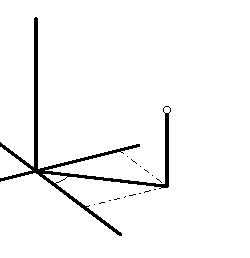
\includegraphics{04cylindrical-coordinates.pdf}}
        \put( 33.19,  31.39){\sffamily\itshape \makebox[0pt][l]{$\theta$}}
    \put( 48.72,  40.03){\sffamily\itshape \makebox[0pt][c]{$r$}}
    \put( 82.16,  52.71){\sffamily\itshape \makebox[0pt][l]{$z$}}
    \put( 52.97,   5.11){\sffamily\itshape $x$}
    \put( 62.61,  57.05){\sffamily\itshape $y$}
    \put( 12.28, 107.01){\sffamily\itshape $z$}

\end{picture}

  \hfill
  \begin{picture} (120.000000,124.068966)(0,0)
    \put(0.0, 0.0){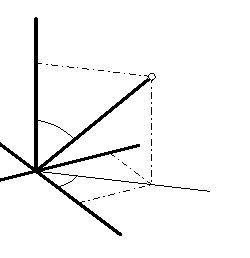
\includegraphics{04spherical-coordinates.pdf}}
        \put( 28.30,  64.10){\sffamily\itshape \makebox[0pt][c]{$\phi$}}
    \put( 36.42,  30.32){\sffamily\itshape \makebox[0pt][c]{$\theta$}}
    \put( 46.07,  59.38){\sffamily\itshape \makebox[0pt][c]{$\rho$}}
    \put( 45.07,  93.30){\sffamily\itshape \makebox[0pt][c]{$\rho\sin\phi$}}
    \put( 52.97,   5.11){\sffamily\itshape $x$}
    \put( 62.61,  48.05){\sffamily\itshape $y$}
    \put( 12.28, 107.01){\sffamily\itshape $z$}

\end{picture}

  \hspace{0.1\textwidth}\null
  \caption{\textbf{Left: } In \emph{cylindrical coordinates} we specify the
  location of a point by its height $z$ above the $xy$-plane, and the
  polar coordinates $(r, \theta)$ of its projection on the $xy$-plane.
  \textbf{Right: } In \emph{spherical coordinates} we specify the location
  of a point by its distance $\rho$ to the origin, the polar angle
  $\theta$ of its projection on the $xy$-plane, and the 
  angle $\phi$ between the $z$-axis and the line segment from the
  point to the origin.}
  \label{fig:04cylindrical-spherical-coords}
\end{figure}

\subsection{Triple integral in cylindrical coordinates}  
Suppose we wanted to find a triple integral
\[
 \liiint_D f(x,y,z)\;dV 
\]
over a domain $D$ which is a ``rectangular block'' in cylindrical coordinates,
i.e.\ suppose $D$ is given by the inequalities
\[
r_0\le r\le r_1, \; z_0\le z\le z_1, \; \theta_0\le \theta\le\theta_1.
\]
Let's try to write it as an iterated integral.  To do this we partition
the region $D$ into many small pieces by dividing the interval $r_0\le
r\le r_1$ into pieces of length $\Delta r$, the interval $z_0 \le z\le
z_1$ into pieces of length $\Delta z$, and interval $\theta_0 \le
\theta\le \theta_1$ into pieces of length $\Delta \theta$.  The whole
region $D$ then gets broken up into small regions in which the radius
is constrained to lie in the interval $(r, r+\Delta r)$, the height
to the interval $(z, z+\Delta z)$ and the polar angle to $(\theta,
\Delta\theta)$.  See Figure~\ref{fig:04cylindrical-volume-element}.
Such a small region is approximately a rectangular block, so that we
can approximate its volume by multiplying the lengths of its sides,
which leads to
\[
\Delta V \approx \Delta r\times r\Delta\theta \times \Delta z.
\]
Arguing as in the case of polar coordinates (see
\S\ref{sec:04double-integrals-in-PC}) we get the following
iterated integral formula for a triple integral over a rectangular
block in cylindrical coordinates:
\begin{equation}
    \iiint\limits_D f(x, y, z) dV
    = 
    \int_{r_0}^{r_1} \int_{z_0}^{z_1} \int_{\theta_0}^{\theta_1}
    f(x, y, z)
    r\;  d\theta\; dz\; dr
    \label{eq:04-tripleint-cylindrical}
\end{equation}
If the function to be integrated is given in terms of the Cartesian
coordinates $x, y, z$, then we first have to rewrite it in terms of
cylindrical coordinates using \eqref{eq:04cylindrical-to-cartesian}.
\begin{figure}[t]
  \begin{picture} (150.000000,204.971429)(0,0)
    \put(0.0, 0.0){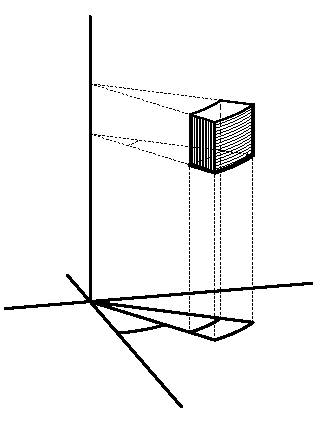
\includegraphics{04cylindrical-volume-element.pdf}}
        \put( 88.06,  10.71){\sffamily\itshape \makebox[0pt][l]{$x$}}
    \put(151.48,  63.99){\sffamily\itshape \makebox[0pt][l]{$y$}}
    \put( 45.29, 186.93){\sffamily\itshape \makebox[0pt][l]{$z$}}
    \put( 97.11, 116.00){\sffamily\itshape \makebox[0pt][c]{$dr$}}
    \put( 79.17, 121.54){\sffamily\itshape \makebox[0pt][c]{$r$}}
    \put(114.60, 118.11){\sffamily\itshape \makebox[0pt][c]{$rd\theta$}}
    \put(123.42, 138.70){\sffamily\itshape \makebox[0pt][l]{$dz$}}
    \put( 68.66,  39.62){\sffamily\itshape \makebox[0pt][l]{$\theta$}}
    \put( 64.38, 141.28){\sffamily\itshape \makebox[0pt][l]{$d\theta$}}

\end{picture}

  \caption{The cylindrical volume element.}
  \label{fig:04cylindrical-volume-element}
\end{figure}


\subsection{Triple integral in spherical coordinates}  
A spherical block is a region $D$ which in spherical coordinates is given by
the inequalities
\[
\rho_0\le \rho\le \rho_1, \; \theta_0\le\theta\le\theta_1,\;
\phi_0\le \phi\le\phi_1
\]
To integrate a function over such a block we divide into many small
spherical blocks.  In each of these blocks $\rho$ increases by
$\Delta\rho$, $\theta$ by $\Delta\theta$, and $\phi$ by $\Delta\phi$.
See Figure~\ref{fig:04spherical-volume-element}.  Any sufficiently small
spherical block is approximately rectangular, and we can therefore
compute its volume by multiplying the lengths of its sides.  If we
carefully look at the drawing on the right in
Figure~\ref{fig:04spherical-volume-element}, then we find that 
\[
\Delta V \approx \rho\Delta\phi\times \rho\sin\phi\Delta\theta \times
\Delta\rho.
\]
\marginpar{\centering\footnotesize\sffamily
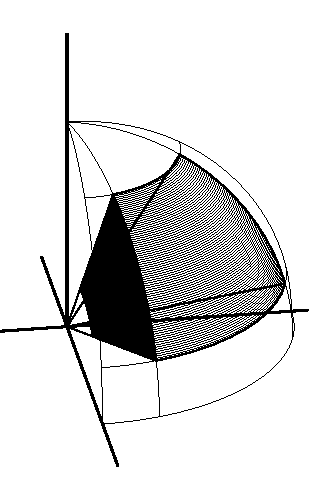
\includegraphics[scale=0.5]{04spherical-block.pdf}\\
A spherical block}%
This leads us to the formula for integration in spherical coordinates:
\begin{equation}
    \iiint\limits_D f(x, y, z) dV
    = 
    \int_{\rho_0}^{\rho_1} \int_{\theta_0}^{\theta_1}
    \int_{\phi_0}^{\phi_1} f(x, y, z)
    \rho^2\sin\phi\; d\phi \; d\theta\; d\rho
    \label{eq:04-tripleint-spherical}
\end{equation}
As in the cases of polar coordinates and cylindrical coordinates we first
have to express the function $f(x, y, z)$ in terms of the variables
$\rho$, $\phi$, and $\theta$, using \eqref{eq:04spherical-to-cartesian}.

\begin{figure}[t]
  \begin{picture} (150.000000,188.057143)(0,0)
    \put(0.0, 0.0){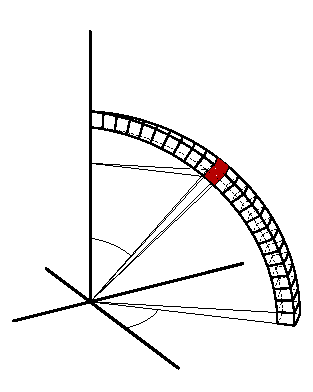
\includegraphics{04spherical-volume-element.pdf}}
        \put( 71.12,  76.09){\sffamily\itshape \makebox[0pt][r]{$\rho$}}
    \put( 56.79,  73.93){\sffamily\itshape \makebox[0pt][c]{$\phi$}}
    \put( 75.12,  31.35){\sffamily\itshape \makebox[0pt][l]{$\theta$}}

\end{picture}
\hfill
  \begin{picture} (150.000000,175.517241)(0,0)
    \put(0.0, 0.0){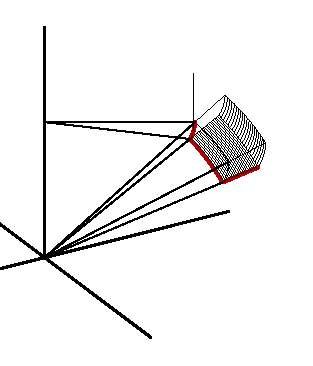
\includegraphics{04spherical-volume-element2.pdf}}
        \put( 98.63,  93.92){\sffamily\itshape \makebox[0pt][r]{$\rho d\phi$}}
    \put( 54.27, 105.01){\sffamily\itshape \makebox[0pt][c]{$\rho\sin\phi$}}
    \put( 92.97, 143.56){\sffamily\itshape \makebox[0pt][c]{$\rho\sin\phi\; d\theta$}}
    \put(117.33,  85.69){\sffamily\itshape \makebox[0pt][l]{$d\rho$}}

\end{picture}

  \caption{\textbf{Left: } a number of small spherical blocks with varying
  $\phi$ but the same $\theta$ and $\rho$ stacked together.
  \textbf{Right: } the volume of a small spherical block is approximately
  the product of the lengths of its sides, so $\Delta V \approx
  \rho^2\sin\phi \Delta\rho\; \Delta\theta\; \Delta\phi$.}
  \label{fig:04spherical-volume-element}
\end{figure}


\subsection{Example -- Rotational Kinetic energy of the Earth}  
The earth is roughly a sphere with radius $a \approx
6400{\rm km}$, which rotates around its axis with angular velocity
$\omega = 2\pi {\rm rad} /{\rm day}$.  Let's assume that the density
of the earth is constant, say, $\mu {\rm kg}/{\rm m}^3$.

To compute the total kinetic energy of the earth we can use formula
\eqref{eq:04kinetic-energy-of-rotating-object}, which tells us that we
have to find
\[
\liiint_{\sf Earth} r^2 \; dV,
\]
where $r$ is the distance to the earth's axis of rotation.

This integral is best computed using spherical coordinates, in which
\[
r = \rho\sin\phi   \quad\text{(see
Figure~\ref{fig:04cylindrical-spherical-coords}, right)}.
\]
Thus the kinetic energy is 
\begin{align*}
  K &= \tfrac12\mu\omega^2 \liiint_{\sf Earth} \rho^2\sin^2\phi \;
  dV\\
  &=
  \tfrac12\mu\omega^2 
  \int_{\phi=0}^\pi \int_{\rho=0}^a \int_{\theta=0}^{2\pi}
  \rho^2\sin^2\phi\;
  \underbrace{\rho^2 \sin\phi \; d\theta\; d\rho\; d\phi}_{dV}.
\end{align*}
After doing the $\theta$ and $\rho$ integrals, we get
\[
K = \pi\mu\omega^2 \frac{a^5}5
\int_0^\pi \sin^3\phi \; d\phi.
\]
This last integral can be done several ways (integrate by parts and
find a reduction formula, or substitute $u = -\cos \phi$).  The result is  
\[
K = \tfrac4{15} \pi \mu \omega^2 a^5.
\]



\section{Problems}  
\problemfont
\begin{multicols}{2}

\problem Describe the following sets  
(given in spherical coordinates):

\subprob All points with $\phi = \pi/6$.
\answer
A cone around the positive $z$ axis, with opening angle $\pi/6.$ 
\endanswer
\subprob All points with $\phi = \pi$.
\answer
The negative half of the $z$ axis.
\endanswer
\subprob All points with $\phi = \pi/2$.
\answer
The $xy$ plane.
\endanswer
\subprob All points with $\theta=\pi/2$ 
\answer
The half of the $yz$ plane which contains the positive $y$ axis, and
which ends at the $z$-axis.
\endanswer

\problem Let $E$ be the part of the sphere with radius $a$, 
centered at the origin, and contained in the first octant

\subprob Describe $E$ in terms of spherical coordinates. 
\answer
$0\leq \theta\le\pi/2$, $0\le \rho\le a$, $0\le\phi\le\pi/2$.
\endanswer

\subprob  Describe $E$ in terms of cylindrical coordinates. 
There are two possible answers, find both.
\answer
$0\le\theta\le\pi/2$, $0\le r\le a$, $0\le z\le \sqrt{a^2-r^2}$, or:

$0\le\theta\le\pi/2$, $0\le z\le a$, $0\le r\le \sqrt{a^2-z^2}$.
\endanswer

\problem Draw the volume elements in cylindrical and in spherical 
coordinates and show how these lead to $dV = rdrd\theta dz$, and
$dV = \rho^2\sin\phi\; d\rho\; d\theta\; d\phi$, respectively.

\answer
Figures \ref{fig:04cylindrical-volume-element} and
\ref{fig:04spherical-volume-element}.
\endanswer

\problem Look at Figure~\ref{fig:04integral-over-sphere}.  
Suppose the grey disc has height $z$, and suppose all points on the
line segment drawn in this disc have the same $y$-coordinate ($y$).

\subprob What are the radii of the two circles drawn in the 
$xy$ plane?
\answer
Large circle has radius $1$, the smaller has radius $\sqrt{1-z^2}$.
\endanswer
\subprob What are the coordinates of the two endpoints of the drawn 
line segment?
\answer
$x=\sqrt{1-y^2-z^2}$ for the point in front, and $x=-\sqrt{1-y^2-z^2}$
for the point in the back (furthest away from you, the viewer).
\endanswer

\problem \textit{The potential energy in a pile of honey. }
If you lift an object to height $h$ above the ground, then the
potential energy you give it is $mgh$, where $m$ is the mass of the
object, and $g$ is the acceleration of gravitation ($g\approx 9.8 {\rm
m}/{\rm sec}^2$).

Suppose that a certain substance occupies a three dimensional region $D$
(think of honey that has just been poured into a jar, see the drawing
which gives a two dimensional side view of the situation).
\begin{center}
  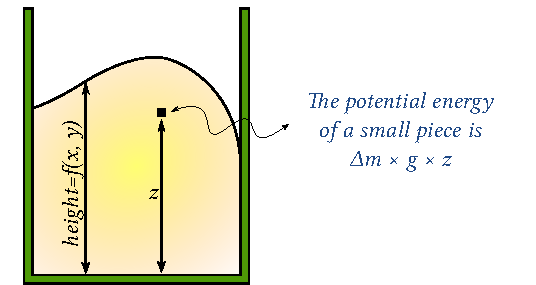
\includegraphics[width=0.4\textwidth]{04jar-of-honey.pdf}
\end{center}
Assuming the base of the jar is an $A\times B$ rectangle, the honey
occupies the region
\begin{multline*}
D = \bigl\{(x,y,z) :\\
0\leq x\leq A, \; 0\leq y\leq B,\\
0\leq z\leq f(x, y)\bigr\}.
\end{multline*}
Here $f(x, y)$ is the height of the honey above the point $(x, y)$ in
the base of the jar.

\subprob What is the potential energy of a small piece 
of the honey at $(x, y, z)$  (assume the density of the honey is
$\mu$, and that this is constant.)  Is your formula an exact
formula?  
\answer
The potential energy is ``mass$\times$height$\times g$''.  The mass of
the small piece of honey is $\Delta m = \mu\times \Delta V$, where
$\Delta V$ is the volume occupied by the small piece of honey.  This
is not an exact formula, but only an approximation, since not all
particles in the small piece of honey have exactly the same height.
However, as one considers smaller and smaller pieces the approximation
gets better.
\endanswer

\subprob Write a volume integral for the total 
(gravitational) potential energy contained in the honey.
\answer
The total potential energy is 
\[
\text{P.E.} = \liiint _D \mu g z \; dV.
\]
Interpretation: this is the total energy that would be released if you
put all the honey at height zero (e.g.\ by pouring it out of the jar
onto the floor.)
\endanswer

\subprob Write your triple integral as an iterated integral, 
and show that you can do the integration in the $z$ direction even if
you don't know the height function $f(x, y)$.
\answer
The iterated integral is
\[
\text{P.E.} = 
\int_{x=0}^A \int_{y=0}^B \int_{z=0}^{f(x, z)} \mu g z \; dz\; dy\;
dx
=
\frac12 \mu g
\int_{x=0}^A \int_{y=0}^B f(x, y)^2 \; dy\; dx.
\]
\endanswer

\problem \textit{The kinetic energy in a tornado.} 

Assume an airmass is whirling around the $z$-axis, and assume that
the wind velocity $v(r)$ only depends on the distance from the $z$-axis.

Assume furthermore that the air has constant density $\mu$.

\subprob Derive a volume integral for the total kinetic energy 
of the airmass in a given region $D$.  (The kinetic energy of an
object of mass $m$ and velocity $v$ is $\frac12 mv^2$.  See the
derivation of the moment of inertia in \S\ref{sec:moment-of-inertia}).
\answer
The kinetic energy in a small region of the airmass is $\frac12 \Delta
m \times v^2$, where $\Delta m$ is the mass of the air in the small
region.  This mass is $\mu\times \Delta V$, with $\Delta V$ the
volume of the small region, so the kinetic energy of the small region
is $\frac 12 \mu \times v^2\times\Delta V$.  Partitioning the
whole airmass, and adding the kinetic energies of all the small pieces
leads to this integral:
\[
\text{K.E.} = \liiint_D \tfrac12\mu v(r)^2\; dV
= \tfrac12\mu \liiint_D v(r)^2\; dV
.\]
\endanswer

\subprob Suppose the velocity is actually given by 
$v(r) = 1/\sqrt{1+r^2}$, the density is $\mu = 1$.  Let $D$ be the
cylinder of height $H$ and radius $R$, with the $z$-axis as its
central axis. How much kinetic energy does the airmass in $D$ have?
(Hint: which coordinates should you use?)
\answer
In cylindrical coordinates the domain is defined by $0\le r\le R$ and
$0< z \le H$, so the integral is
\[
\text{K.E.}
=
\frac 12
\int_{\theta=0}^{2\pi}\int_{z=0}^{H}\int_{r=0}^R
\frac{r}{1+r^2}\; dr\; dz\; d\theta
=
\frac{\pi}{2}H\ln\bigl(1+R^2\bigr).
\]
\endanswer

\problem For each of the following iterated integrals, 
describe and draw the domain of integration.  Then compute the
integral.

\subprob$\DS\int_{0}^{2}\int_{-1}^{x^2}\int_{1}^{y} 
xyz \,dz\,dy\,dx$.
\answer
$623/60$
\endanswer

\subprob$\DS\int_{0}^{1}\int_{0}^{x}\int_{0}^{\ln y} 
e^{x+y+z}\,dz\,dy\,dx$.
\answer
$-3e^2/4+2e-3/4$
\endanswer

\subprob
$\DS\int_{0}^{\pi/2}\int_{0}^{\sin\theta}\int_{0}^{r\cos\theta}
r^2\,dz\,dr\,d\theta$.
\answer
$1/20$
\endanswer

\subprob 
$\DS\int_{0}^{\pi}\int_{0}^{\sin\theta}\int_{0}^{r\sin\theta}
r\cos^2\theta\,dz\,dr\,d\theta$.
\answer
$\pi/48$
\endanswer

\subprob$\DS\int_{0}^{1}\int_{0}^{y^2}\int_{0}^{x+y} 
x\,dz\,dx\,dy$.
\answer
$11/84$
\endanswer

\subprob$\DS\int_{1}^{2}\int_{y}^{y^2}\int_{0}^{\ln(y+z)} 
e^x\,dx\,dz\,dy$.
\answer
$151/60$
\endanswer


\problem Find the mass of a cube with edge length 2 and density equal 
to the square of the distance from one corner.
\answer
$32$
\endanswer

\problem Find the mass of a cube with edge length 2 and density equal 
to the square of the distance from one edge.
\answer
$64/3$
\endanswer
\[
\diamondsuit
\]

If a mass is distributed throughout a region $D$ with density
$\mu(x, y, z)$, then, by definition the coordinates $(X,Y,Z)$
of the \emph{center of mass} 
\[
X \stackrel{\rm def}{=} \frac{\iiint_D x\mu(x, y, z))\; dV}{\text{Mass of }D},
\]
and similarly for $Y$ and $Z$.

\problem An object occupies the volume of the upper hemisphere of  
$x^2+y^2+z^2=4$ and has density $z$ at $(x,y,z)$. Find the center of mass.

\answer
$\bar x=\bar y=0$, $\bar z=16/15$
\endanswer

\problem An object occupies the volume of the pyramid with corners at  
$(1,1,0)$, $(1,-1,0)$, $(-1,-1,0)$, $(-1,1,0)$, and $(0,0,2)$ and has
density $x^2+y^2$ at $(x,y,z)$. Find the center of mass.
\answer
$\bar x=\bar y=0$, $\bar z=1/3$
\endanswer

\problem Let $z=f(x, y)$ be a function on some domain $D$, 
and assume that $D$ is split into two parts:  $D_+$, on which
$f\geq 0$, and $D_-$, on which $f(x, y)<0$.

Let $V_+$ be the volume of the region beneath the graph of $f$ and above the
domain $D_+$ in the $xy$-plane, and, similarly, let $V_-$ be the
volume of the region above the graph of $f$ and beneath the region
$D_-$ in the $xy$-plane.

Reminder:  \emph{volumes are never negative}, so both $V_+\ge0$ and
$V_-\ge0$.

\subprob Express the following integrals in terms of $V_+$ and 
$V_-$:
\begin{align*}
  I &= \iint_{D_+}f(x, y)\; dA, \\
  J &= \iint_{D_-}f(x, y)\; dA \\
  K &= \iint_{D}f(x, y)\; dA \\
  L &= \iint_{D}|f(x, y)|\; dA.
\end{align*}
\answer
$I=V_+$, $J= -V_-$ (note the minus sign),
$K= V_+-V_-$, $L = V_+ + V_-$.
\endanswer

\subprob Find the region $E$ in three dimensional space for which
\[
\DS\liiint_{E} (1-x^2-y^2-z^2) \; \dV
\]
is a maximum.  [Hint: Suppose $E$ is some region; consider then 
what happens to the integral if you make $E$ larger by adding on a
piece.]






\problem Evaluate
\[
\int_{0}^{1}\int_{0}^{x}\int_{0}^{\sqrt{x^2+y^2}} 
{(x^2+y^2)^{3/2}\over x^2+y^2+z^2}\,dz\,dy\,dx.  
\]
\answer
$\pi/12$
\endanswer

\problem Evaluate $\DS\iiint x^2\,\dV $ 
over the interior of the cylinder $x^2+y^2=1$ between $z=0$ and $z=5$.
\answer
$5\pi/4$
\endanswer

\problem Evaluate $\DS\iiint xy\,\dV $ 
over the interior of the cylinder $x^2+y^2=1$ between $z=0$ and $z=5$.
\answer
$0$
\endanswer

\problem Evaluate $\DS\iiint z\,\dV $ 
over the region above the $x$-$y$ plane, inside $x^2+y^2-2x=0$ and
under $x^2+y^2+z^2=4$.
\answer
$5\pi/4$
\endanswer

\problem Evaluate $\DS\iiint yz\,\dV $ 
over the region in the first octant, inside $x^2+y^2-2x=0$ and 
under $x^2+y^2+z^2=4$.
\answer
$4/5$
\endanswer

\problem Evaluate $\DS\iiint x^2+y^2\,\dV $ 
over the interior of $x^2+y^2+z^2=4$.
\answer
$256\pi/15$
\endanswer

\problem Evaluate $\DS\iiint \sqrt{x^2+y^2}\,\dV $ 
over the interior of $x^2+y^2+z^2=4$.
\answer
$4\pi^2$
\endanswer

\problem Find the mass of a right circular cone of height $h$ and 
base radius $a$ if the density is proportional to the distance from
the base.
\answer
$\pi kh^2a^2/12$
\endanswer

\problem Find the mass of a right circular cone of height $h$ and 
base radius $a$ if the density is proportional to the distance from
its axis of symmetry.
\answer
$\pi kha^3/6$
\endanswer

\problem An object occupies the region inside the unit sphere at the 
origin, and has density equal to the distance from the $x$-axis. Find
the mass.
\answer
$\pi^2/4$
\endanswer

\problem An object occupies the region inside the unit sphere at the 
origin, and has density equal to the square of the distance from the
origin. Find the mass.
\answer
$4\pi/5$
\endanswer

\problem An object occupies the region between the unit sphere at the 
origin and a sphere of radius 2 with center at the origin, and has
density equal to the distance from the origin. Find the mass.
\answer
$15\pi$
\endanswer





\end{multicols}
\noproblemfont



%%% Local Variables:
%%% mode: latex
%%% TeX-master: "free234"
%%% End:
